\section{Одноканальная система в форме вход-выход}

Рассмотрим следующее дифференциальное уравнение:
\begin{equation}
    \label{eq:source_eq}
    \dddot{y} + a_2 \ddot{y} + a_1 \dot{y} + a_0 y = b_2 \ddot{u} + b_1 \dot{u} + b_0 u
\end{equation}

Перепишем его в операторной форме:
\begin{equation}
    \label{eq:eq2}
    p^3 y + a_2 p^2 y + a_1 p y + a_0 y = b_2 p^2 u + b_1 p u + b_0 u
\end{equation}

Упростим уравнение, выразив $y$:
\begin{equation}
    \label{eq:final_eq}
    y = \frac{1}{p}(b_2 u - a_2 y + \frac{1}{p}(b_1 u - a_1 y + \frac{1}{p}(b_0 u - a_0 y)))
\end{equation}

Теперь, имея данное уравнение, можно построить схему моделирования в Matlab Simulink (рис. \ref{fig:model1}).

\begin{figure}[ht!]
    \centering
    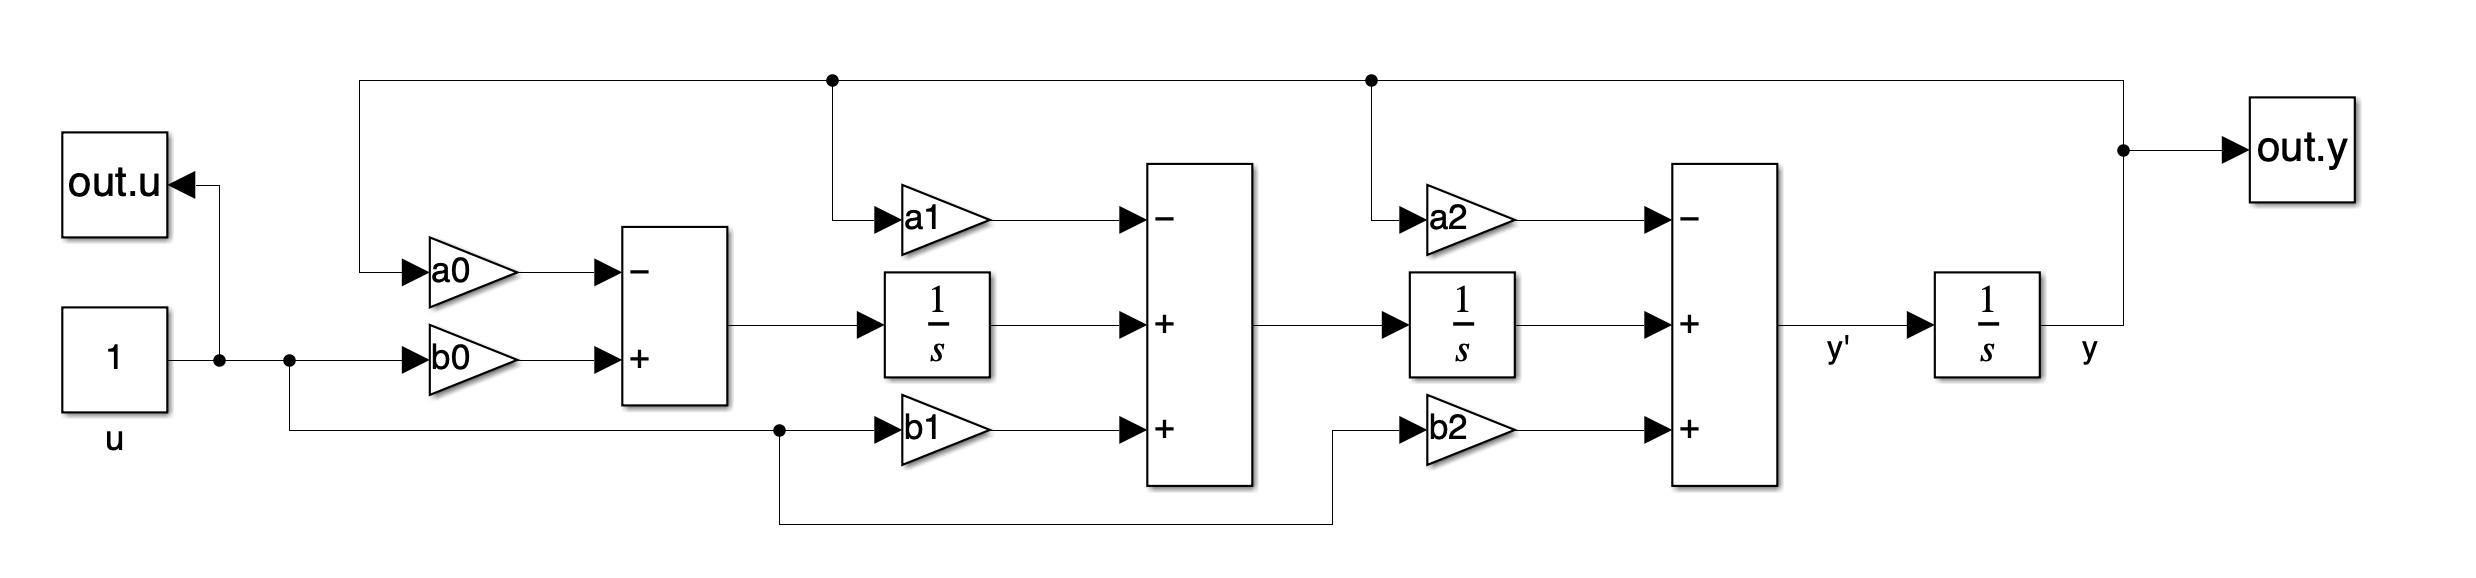
\includegraphics[width=\textwidth]{media/system.png}
    \caption{Схема моделирования одноканальной системы в форме вход-выход}
    \label{fig:model1}
\end{figure}

При этом, начальные условия $\dddot{y}(0) = 0, \ddot{y}(0) = 0, \dot{y}(0) = 0$ задаются в блоках \textit{Integrator}.

Промоделировав данную систему получим графики $y(t)$ и $u(t)$ (рис. \ref{fig:yt}, \ref{fig:ut}).

\begin{figure}
    \centering
    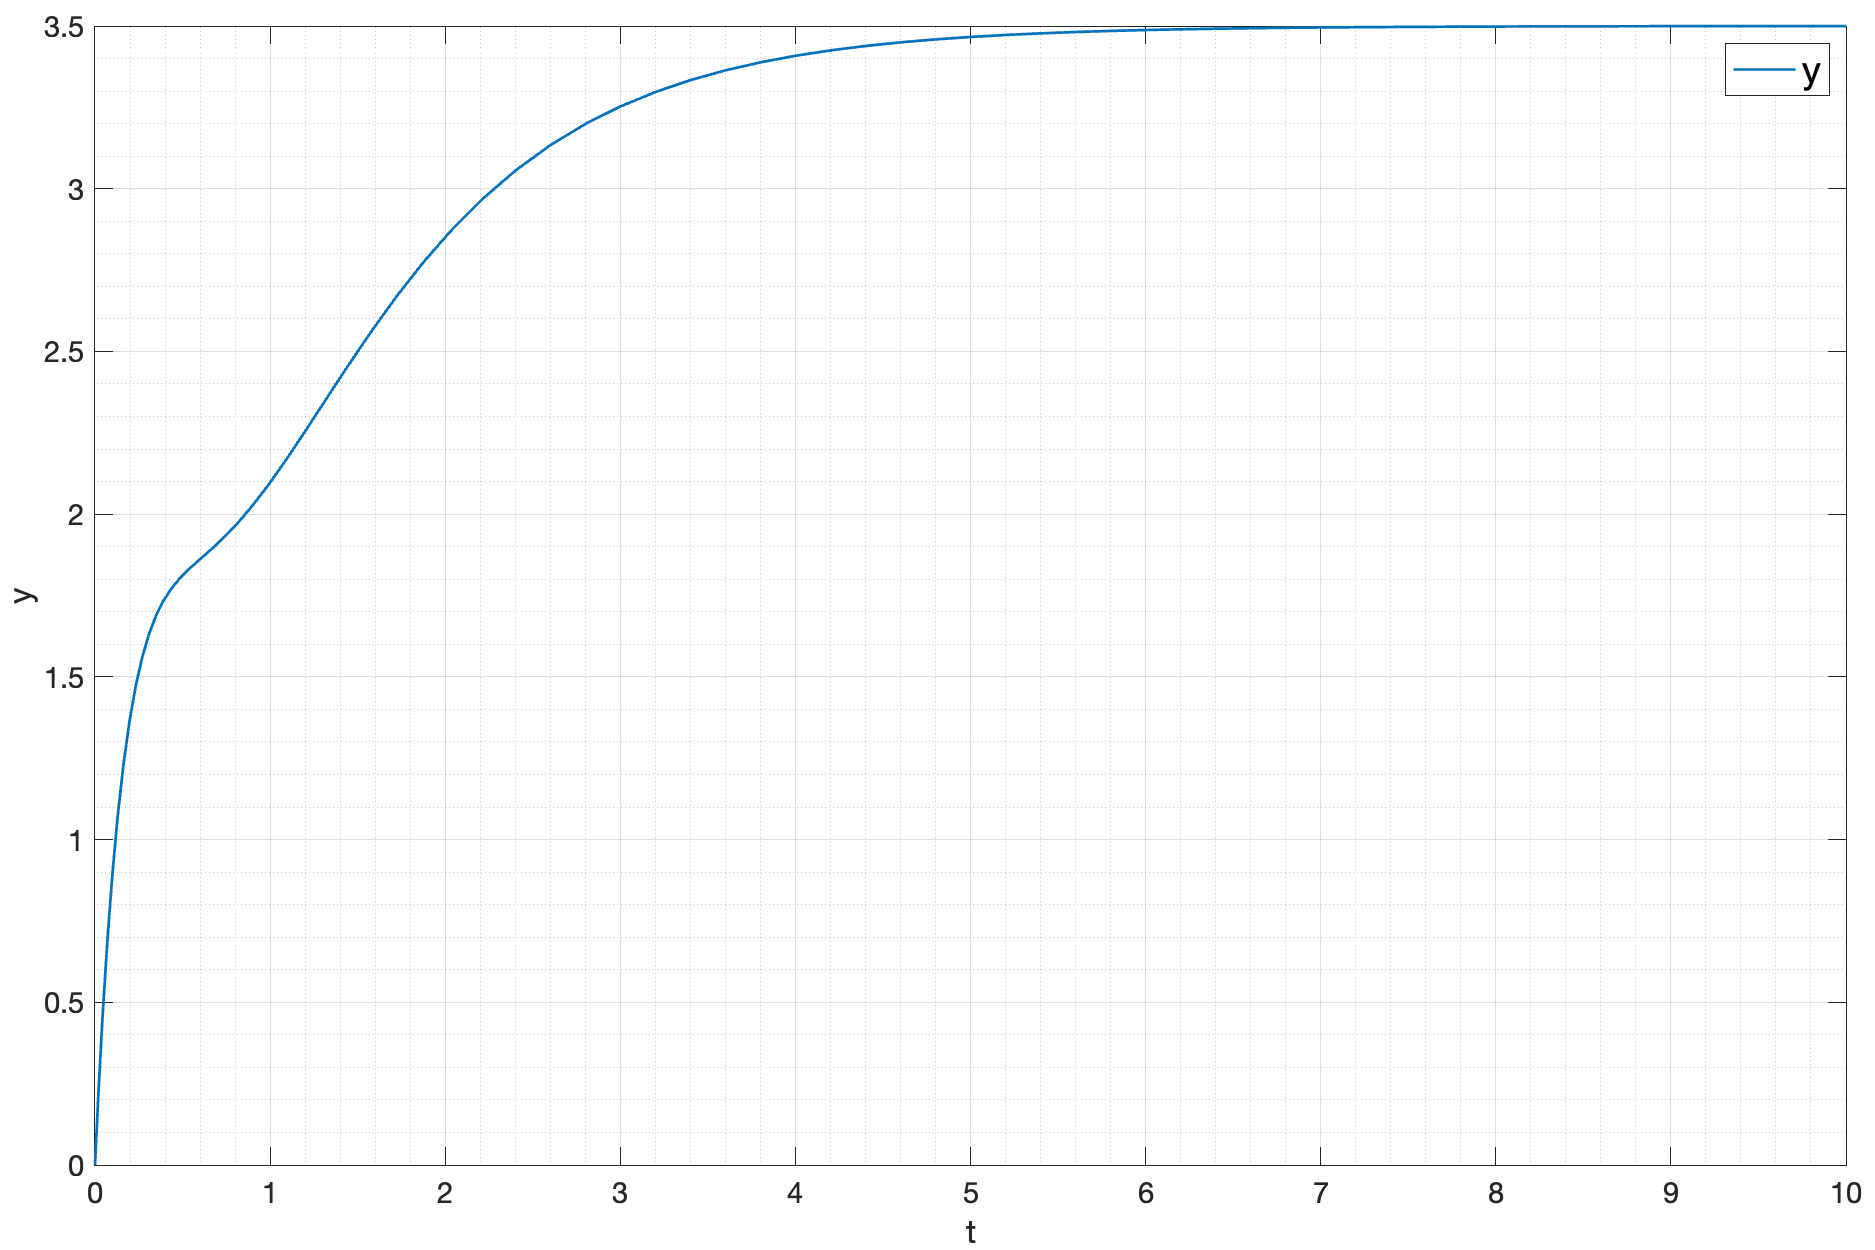
\includegraphics[width=\textwidth]{media/sys1_y(t).png}
    \caption{График $y(t)$}
    \label{fig:yt}
\end{figure}

\begin{figure}
    \centering
    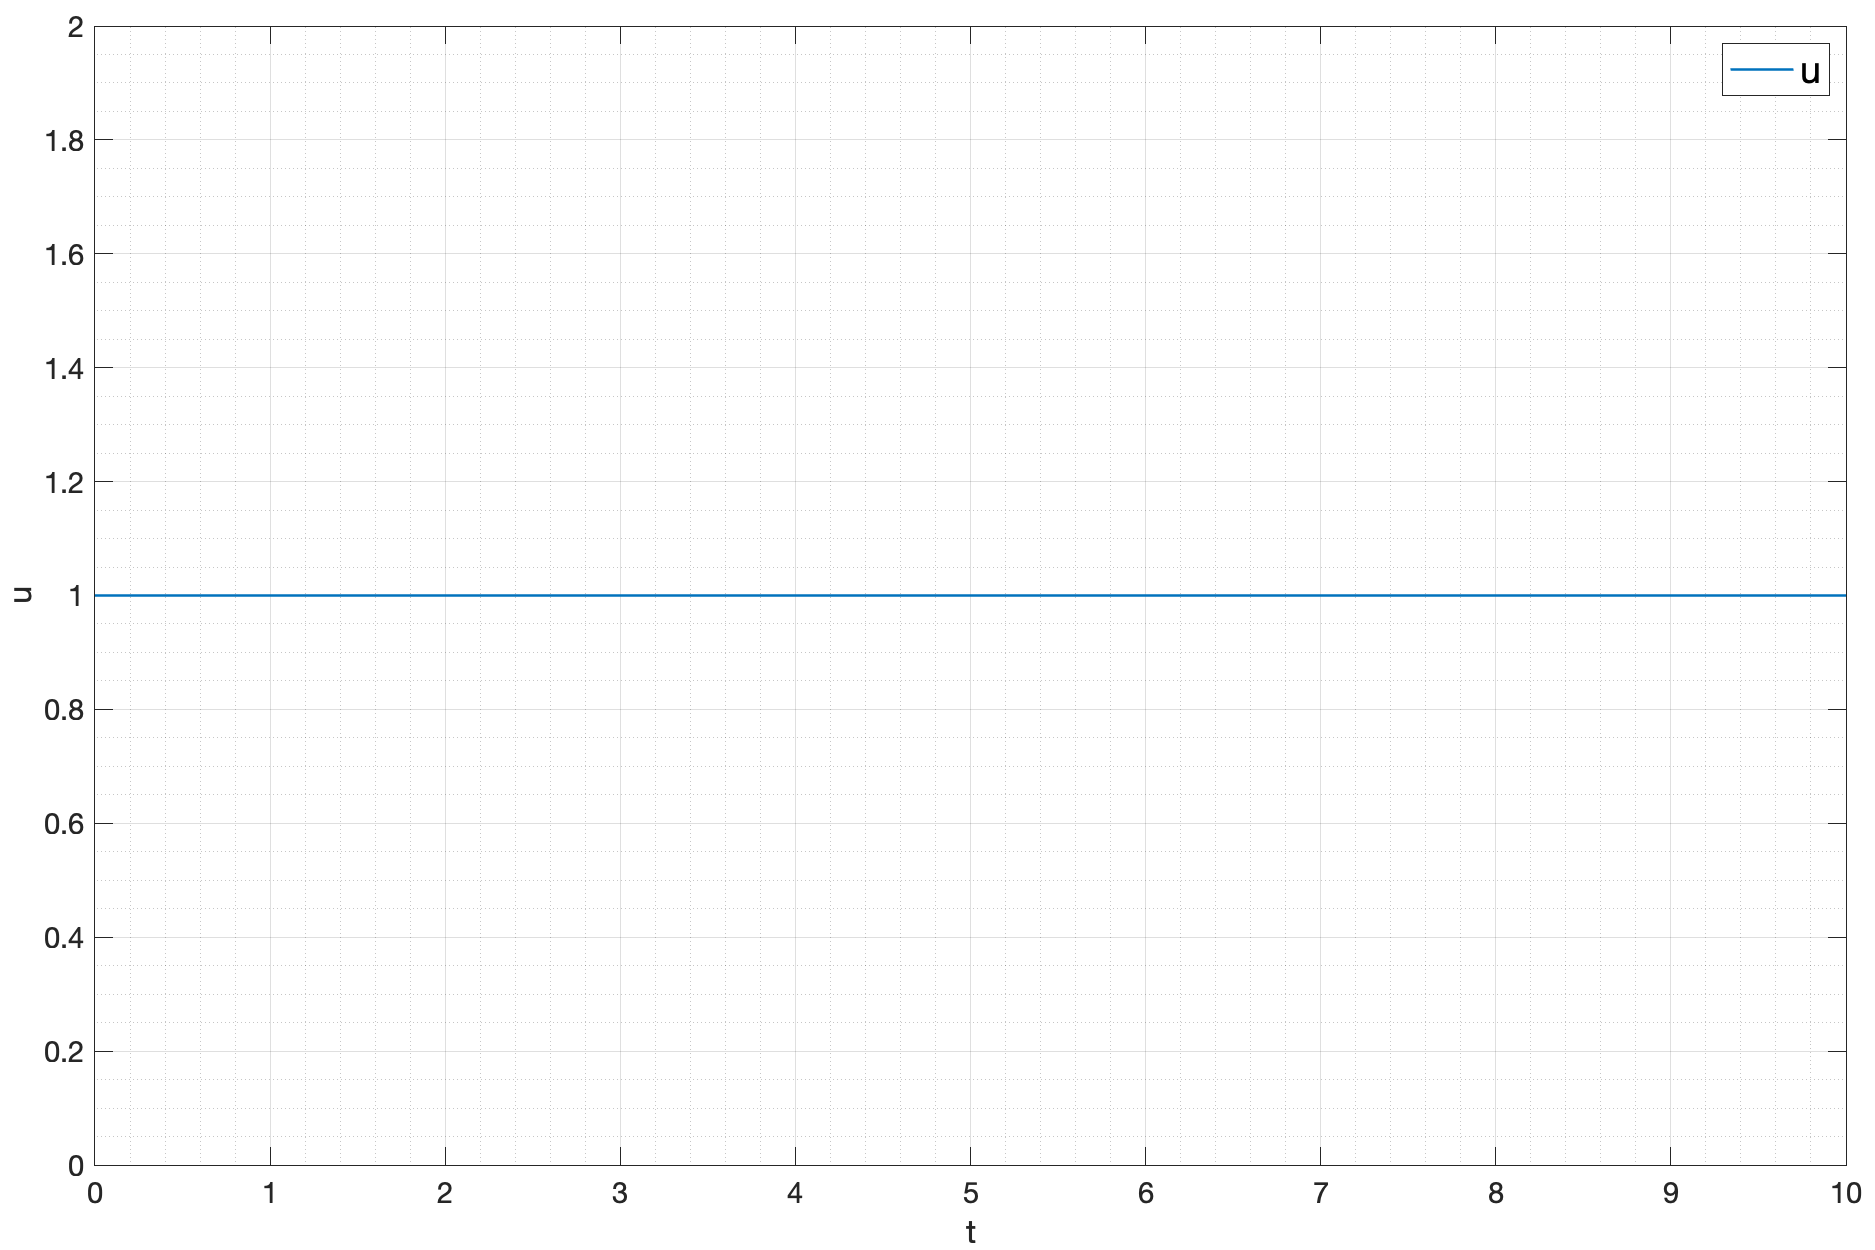
\includegraphics[width=\textwidth]{media/sys1_u(t).png}
    \caption{График $u(t)$}
    \label{fig:ut}
\end{figure}

\FloatBarrier{}

\section{Переход от формы В-В к форме В-С-В}

В общем виде наблюдаемая форма для системы третьего порядка имеет вид:
\begin{equation}
    \begin{cases}
        \dot{x}_1 = a_{11} x_1 + a_{12} x_2 + a_{13} x_3 + b_1 u \\
        \dot{x}_2 = a_{21} x_1 + a_{22} x_2 + a_{23} x_3 + b_2 u \\
        \dot{x}_3 = a_{31} x_1 + a_{32} x_2 + a_{33} x_3 + b_3 u \\
        y = c_1 x_1 + c_2 x_2 + c_3 x_3
    \end{cases}
\end{equation}
где $x_1, x_2, x_3$ -- вектор состояния, $y$ -- выходной сигнал, $u$ -- входной сигнал.

Или, в матричной форме:
\begin{equation}
    \begin{cases}
        \dot{x} = Ax + Bu \\
        y = Cx
    \end{cases}
\end{equation}

Для уравнения \ref{eq:source_eq} перейдем к форме В-С-В. Для этого определим передаточную функцию $W(p)$:
\begin{equation}
    W(p) = \frac{Y(p)}{U(p)} = \frac{b_2 p^2 + b_1 p + b_0}{p^3 + a_2 p^2 + a_1 p + a_0} + S
\end{equation}
где $S$ -- общее решение однородного уравнения $\dddot{y} + a_2\ddot{y} + a_1\dot{y} + a_0y = 0$. Так как у нас нет начальных условий, то $S = 0$.

\subsection{Каноническая наблюдаемая форма}

Для перехода от формы В-В к форме В-С-В воспользуемся следующими соотношениями:
\begin{equation}
    A = \begin{bmatrix}
        0 & 1 & 0 \\
        0 & 0 & 1 \\
        -a_0 & -a_1 & -a_2
    \end{bmatrix},~~~
    B = \begin{bmatrix}
        0 \\
        0 \\
        1
    \end{bmatrix},~~~
    C = \begin{bmatrix}
        b_0 & b_1 & b_2
    \end{bmatrix}
\end{equation}

Таким образом, получаем следующую систему:
\begin{equation}
    \begin{cases}
        \dot{x}_1 = x_2 \\
        \dot{x}_2 = x_3 \\
        \dot{x}_3 = -a_2 x_3 - a_1 x_2 - a_0 x_1 + b_0 u \\
        y = b_2 x_3 + b_1 x_2 + b_0 x_1
    \end{cases}
\end{equation}

Построим схему моделирования в Matlab Simulink (рис. \ref{fig:model2}).
\begin{figure}[ht!]
    \centering
    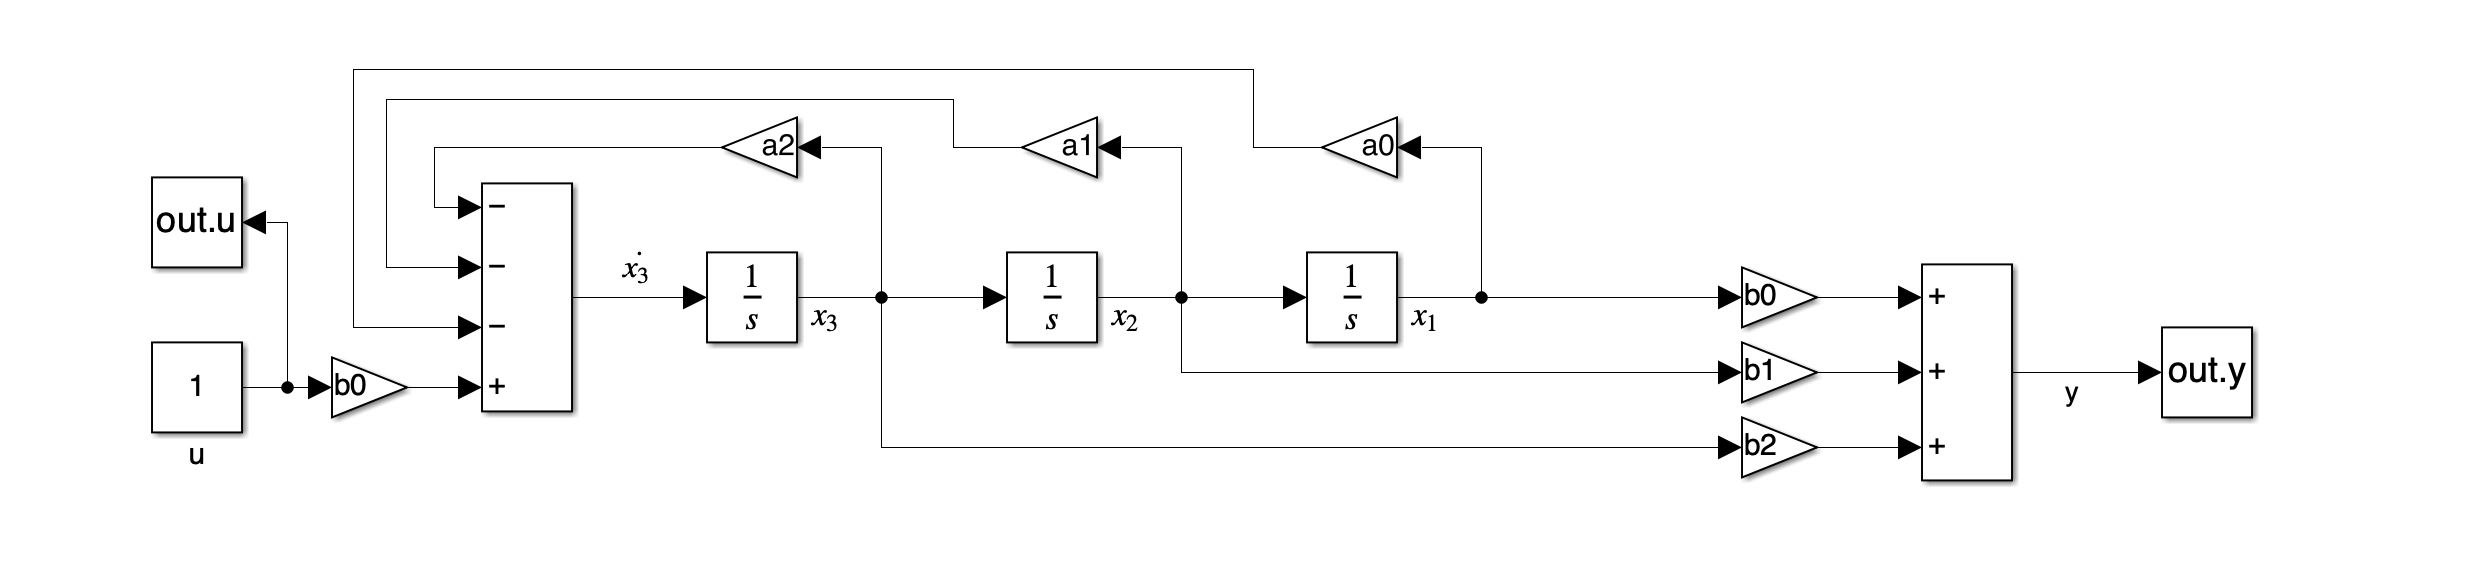
\includegraphics[width=\textwidth]{media/system2.png}
    \caption{Схема моделирования одноканальной системы в форме В-С-В (каноническая наблюдаемая форма)}
    \label{fig:model2}
\end{figure}

Промоделировав данную систему получим график $y(t)$ (рис. \ref{fig:yt2}).
\begin{figure}[ht!]
    \centering
    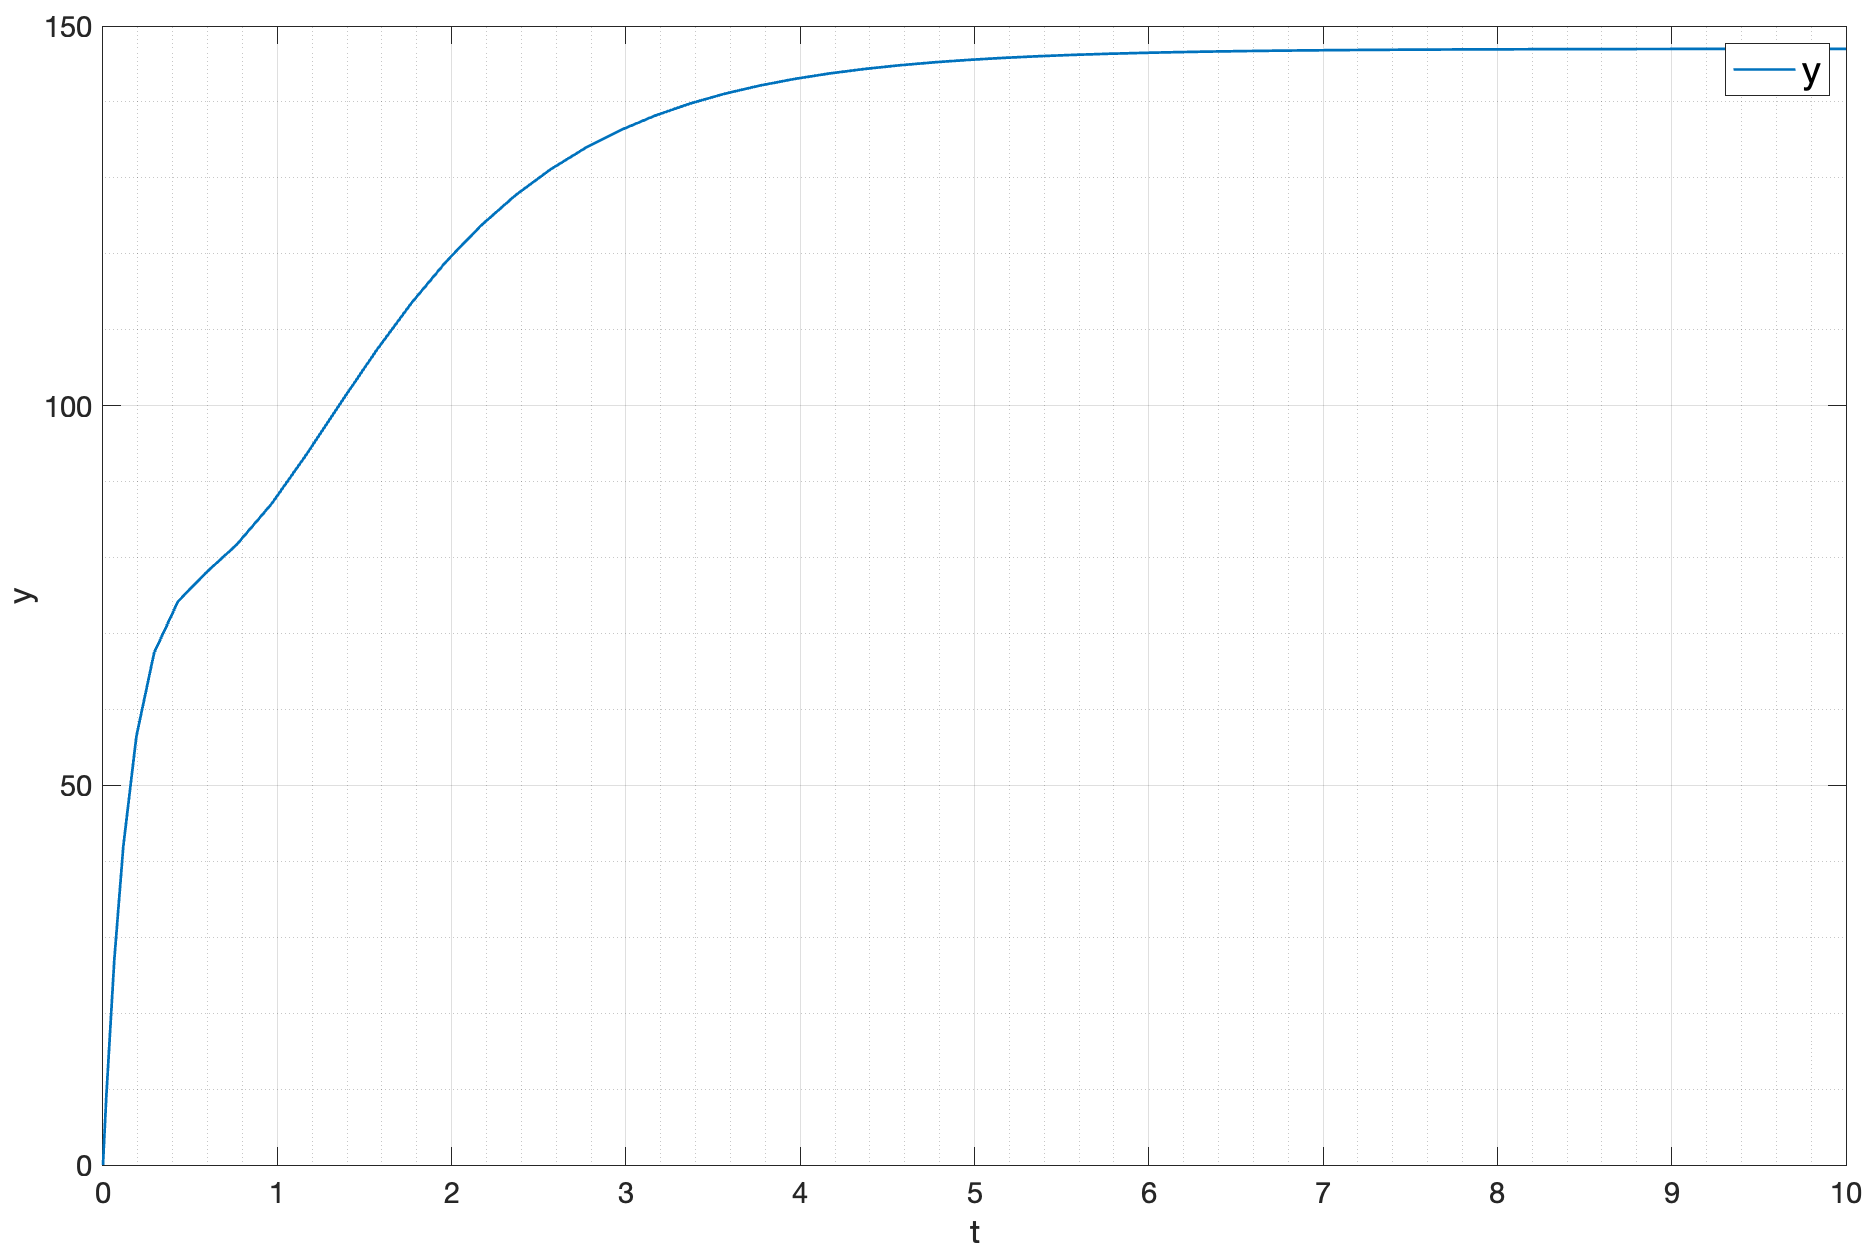
\includegraphics[width=\textwidth]{media/sys2_y(t).png}
    \caption{График $y(t)$}
    \label{fig:yt2}
\end{figure}

На сравнительном графике $y(t)$ для системы в форме В-В и В-С-В (рис. \ref{fig:cmp_sys1_sys2}), видно, что выходной сигнал 
для системы в форме В-С-В по амплитуде больше, чем для системы в форме В-В, но по форме сигналы совпадают. Убедиться в этом 
можно сравнив масштабированные графики (рис. \ref{fig:cmp_sys1_sys2_scaled}).

\begin{figure}[ht!]
    \centering
    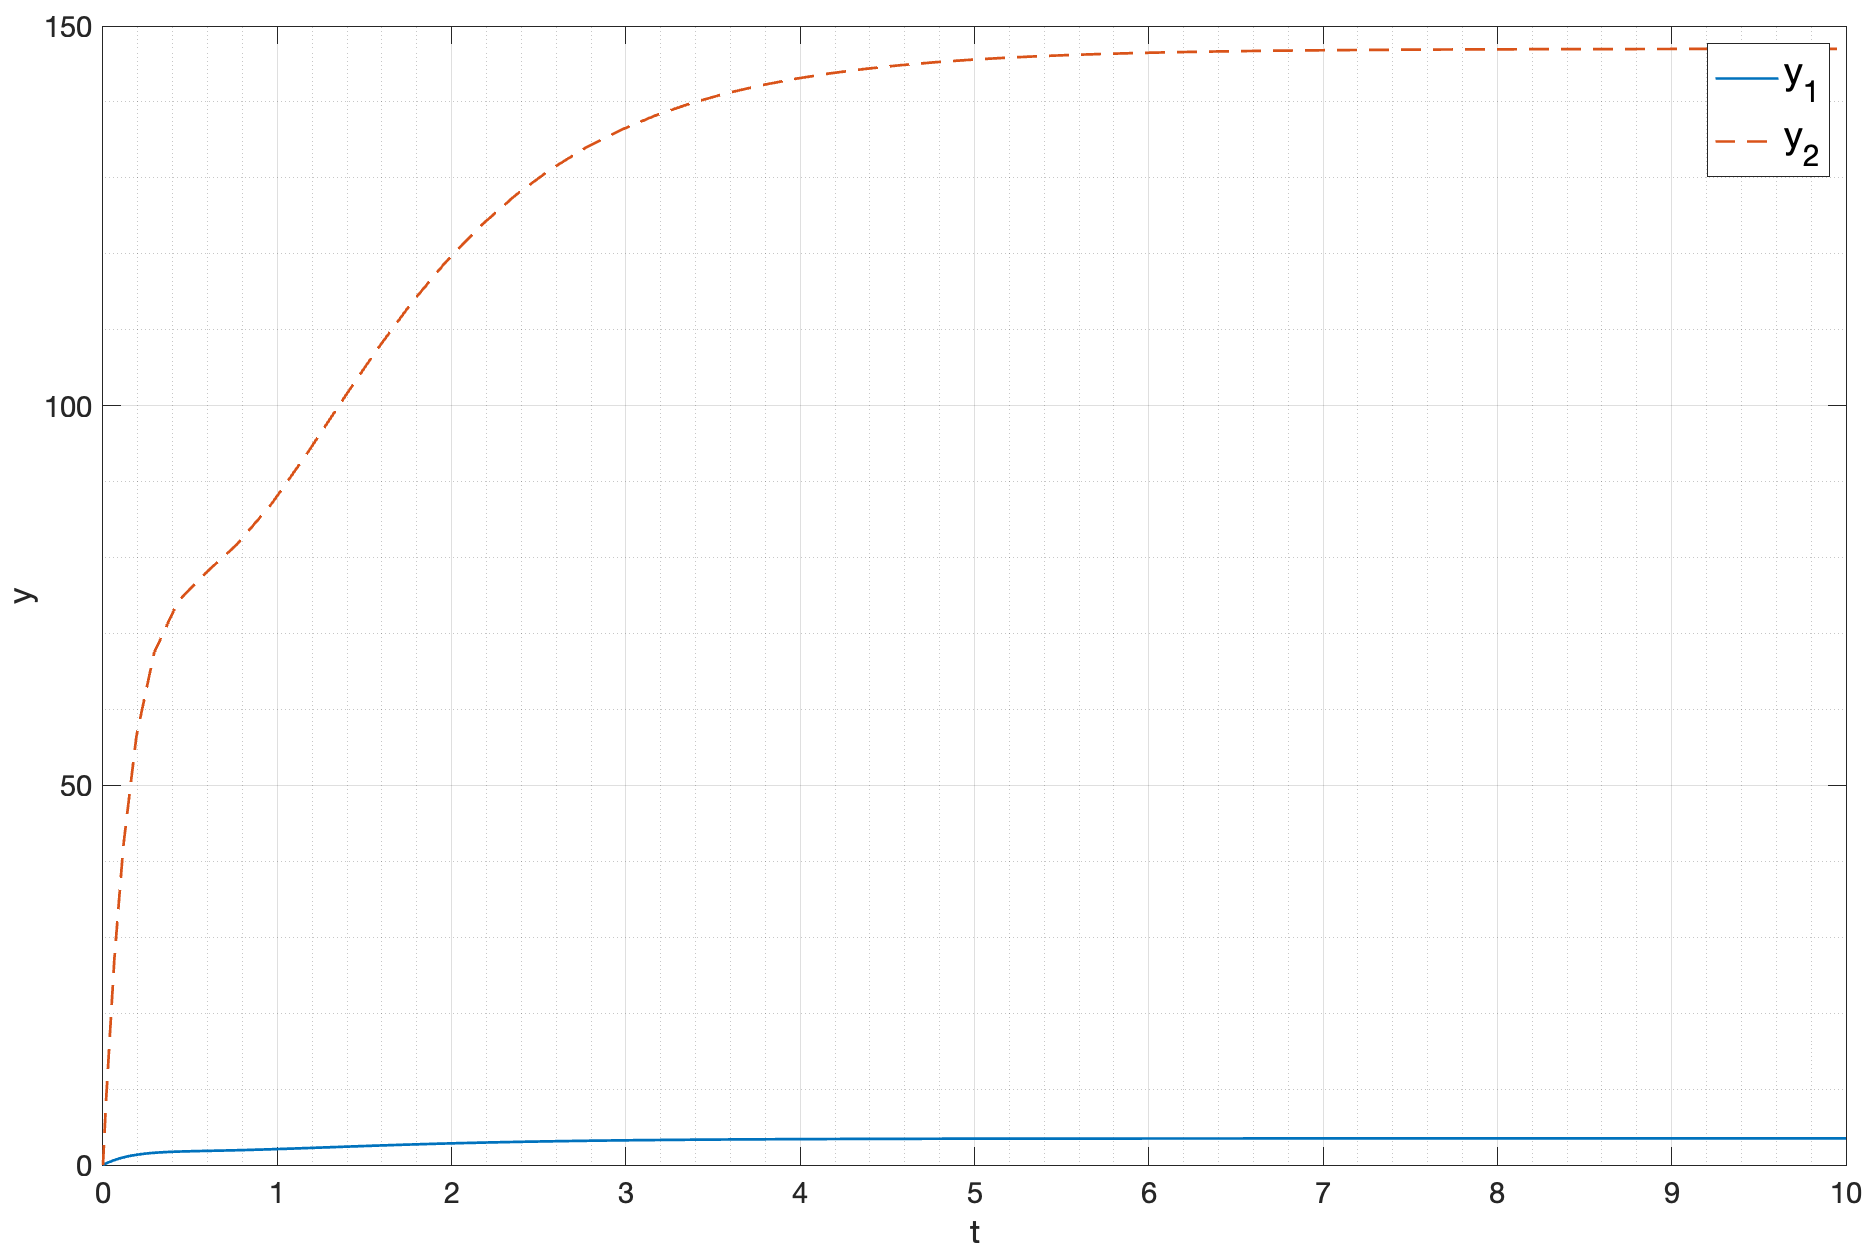
\includegraphics[width=\textwidth]{media/cmp_sys1_sys2.png}
    \caption{Сравнительный график $y(t)$ для системы в форме В-В и В-С-В}
    \label{fig:cmp_sys1_sys2}
    где $y_1(t)$ -- график для системы в форме В-В, $y_2(t)$ -- график для системы в форме В-С-В.
\end{figure}

\begin{figure}[ht!]
    \centering
    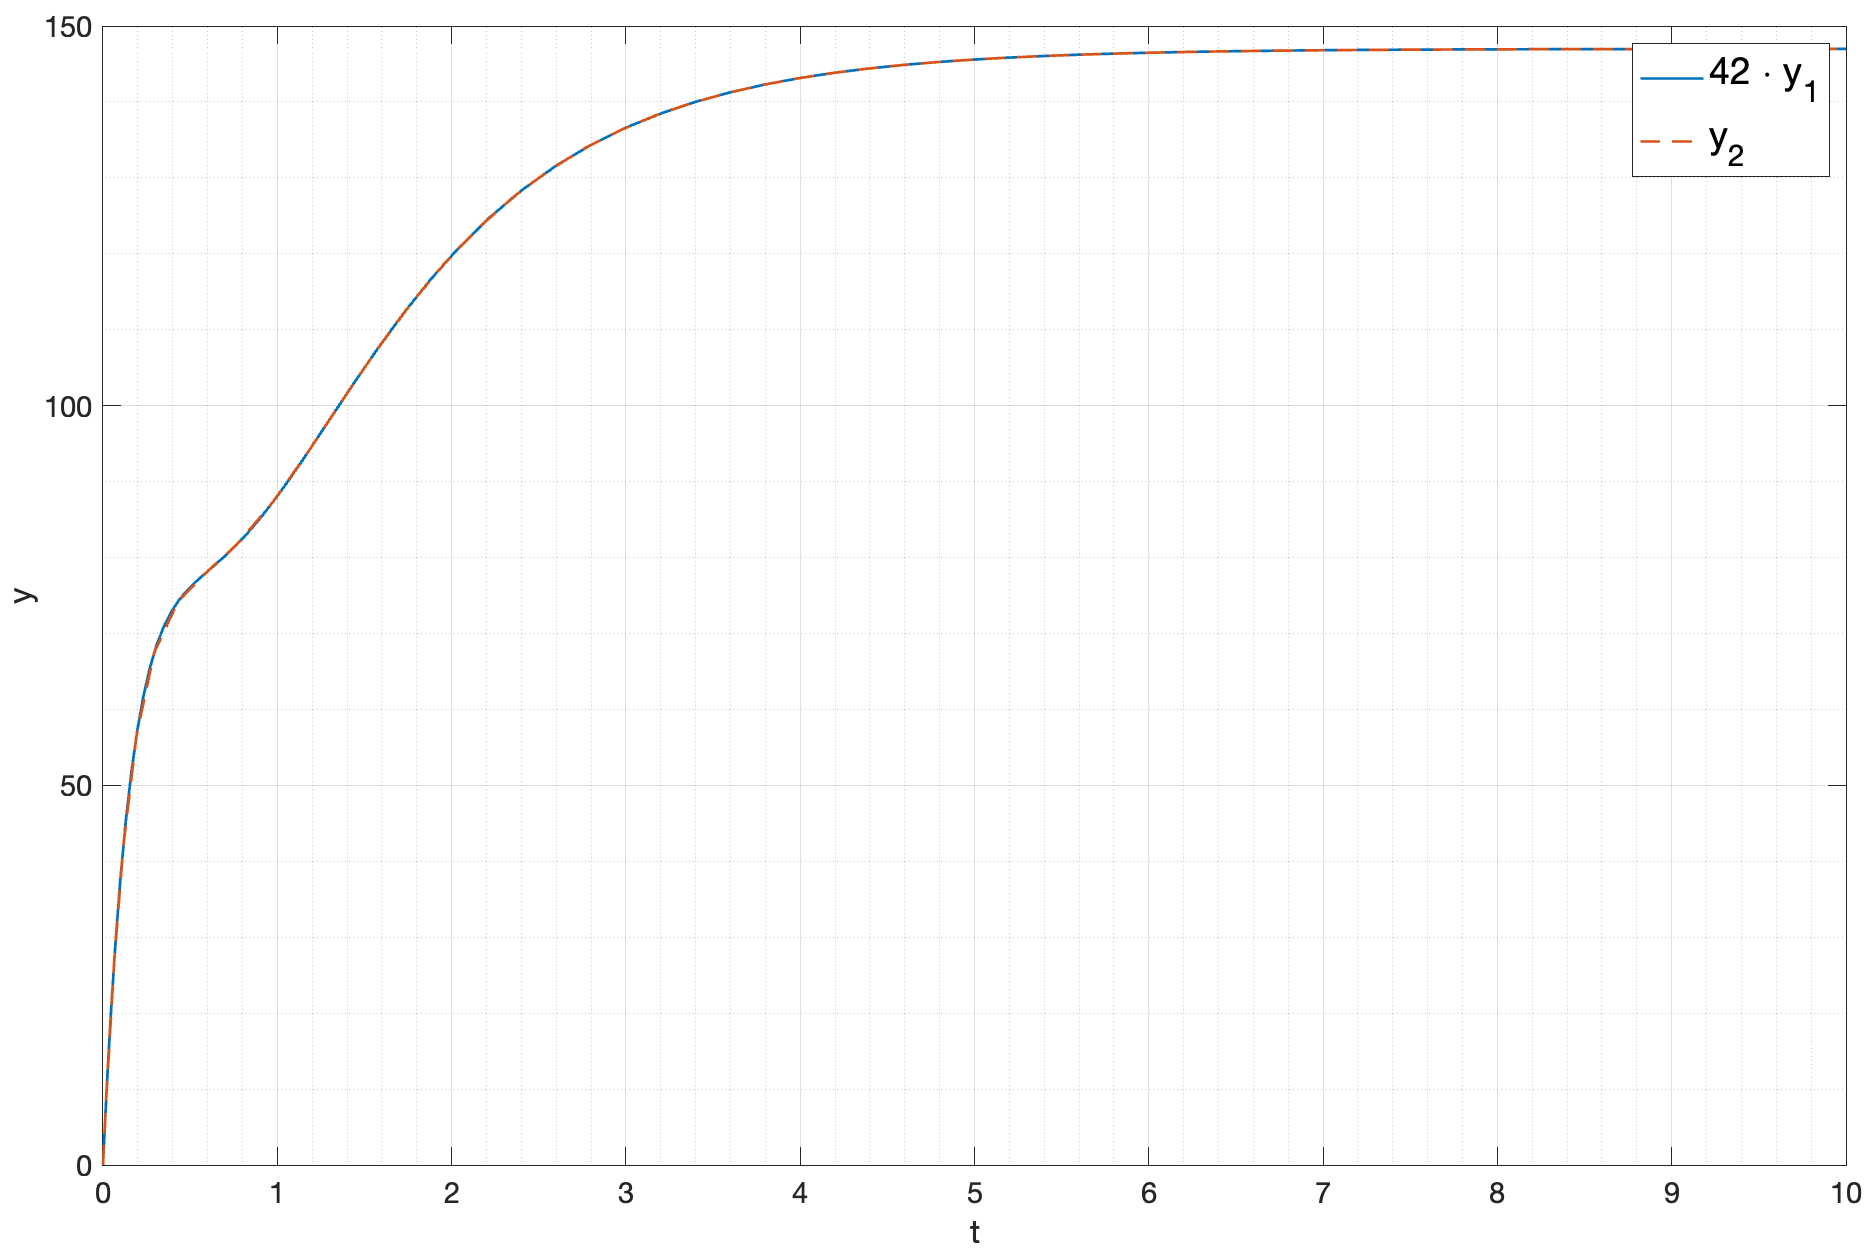
\includegraphics[width=\textwidth]{media/cmp_sys1_sys2_scaled.png}
    \caption{Сравнительный график $y(t)$ для системы в форме В-В и В-С-В (масштабированный)}
    \label{fig:cmp_sys1_sys2_scaled}
\end{figure}

\FloatBarrier

\subsection{Каноническая управляемая форма}

Для перехода от формы В-В к форме В-С-В (каноническая управляемая форма) воспользуемся следующими соотношениями:
\begin{equation}
    A = \begin{bmatrix}
        0 & 0 & -a_0 \\
        1 & 0 & -a_1 \\
        0 & 1 & -a_2
    \end{bmatrix},~~~
    B = \begin{bmatrix}
        b_1 \\
        b_2 \\
        b_3
    \end{bmatrix},~~~
    C = \begin{bmatrix}
        0 & 0 & 1
    \end{bmatrix}
\end{equation}

Таким образом, получаем следующую систему:
\begin{equation}
    \begin{cases}
        \dot{x}_1 = -a_0 x_3 + b_0 u\\
        \dot{x}_2 = -a_1 x_3 + x_1 + b_1 u\\
        \dot{x}_3 = -a_2 x_3 + x_2 + b_2 u \\
        y = x_3
    \end{cases}
\end{equation}

Построим схему моделирования в Matlab Simulink (рис. \ref{fig:model3}).

\begin{figure}[ht!]
    \centering
    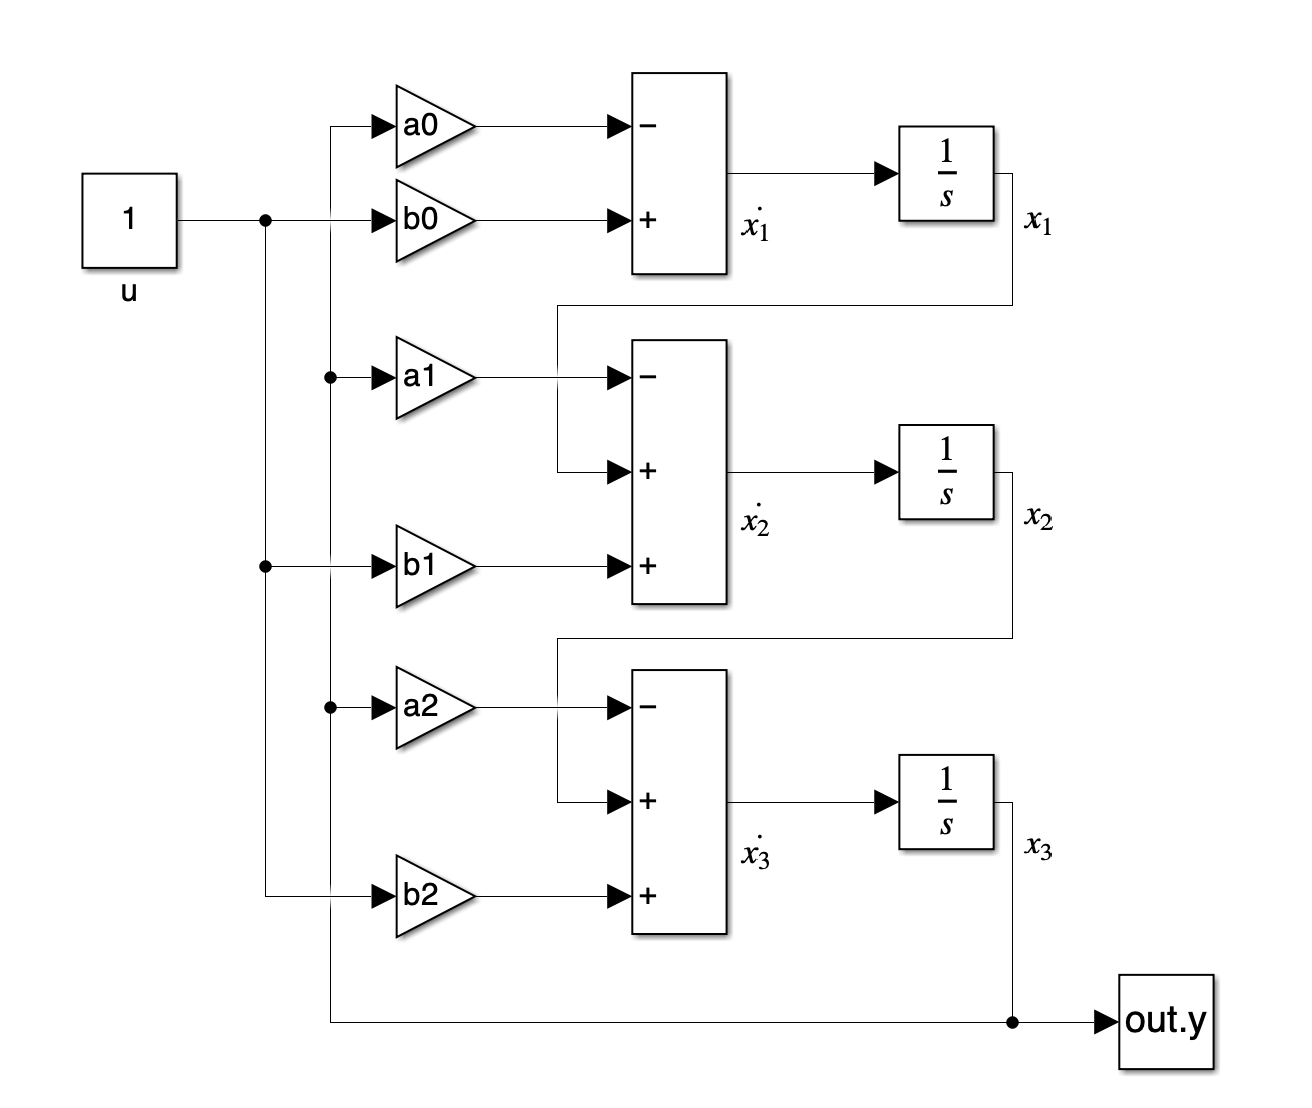
\includegraphics[width=0.7\textwidth]{media/system3.png}
    \caption{Схема моделирования одноканальной системы в форме В-С-В (каноническая управляемая форма)}
    \label{fig:model3}
\end{figure}


Промоделировав данную систему получим график $y(t)$ (рис. \ref{fig:yt3}).
\begin{figure}[ht!]
    \centering
    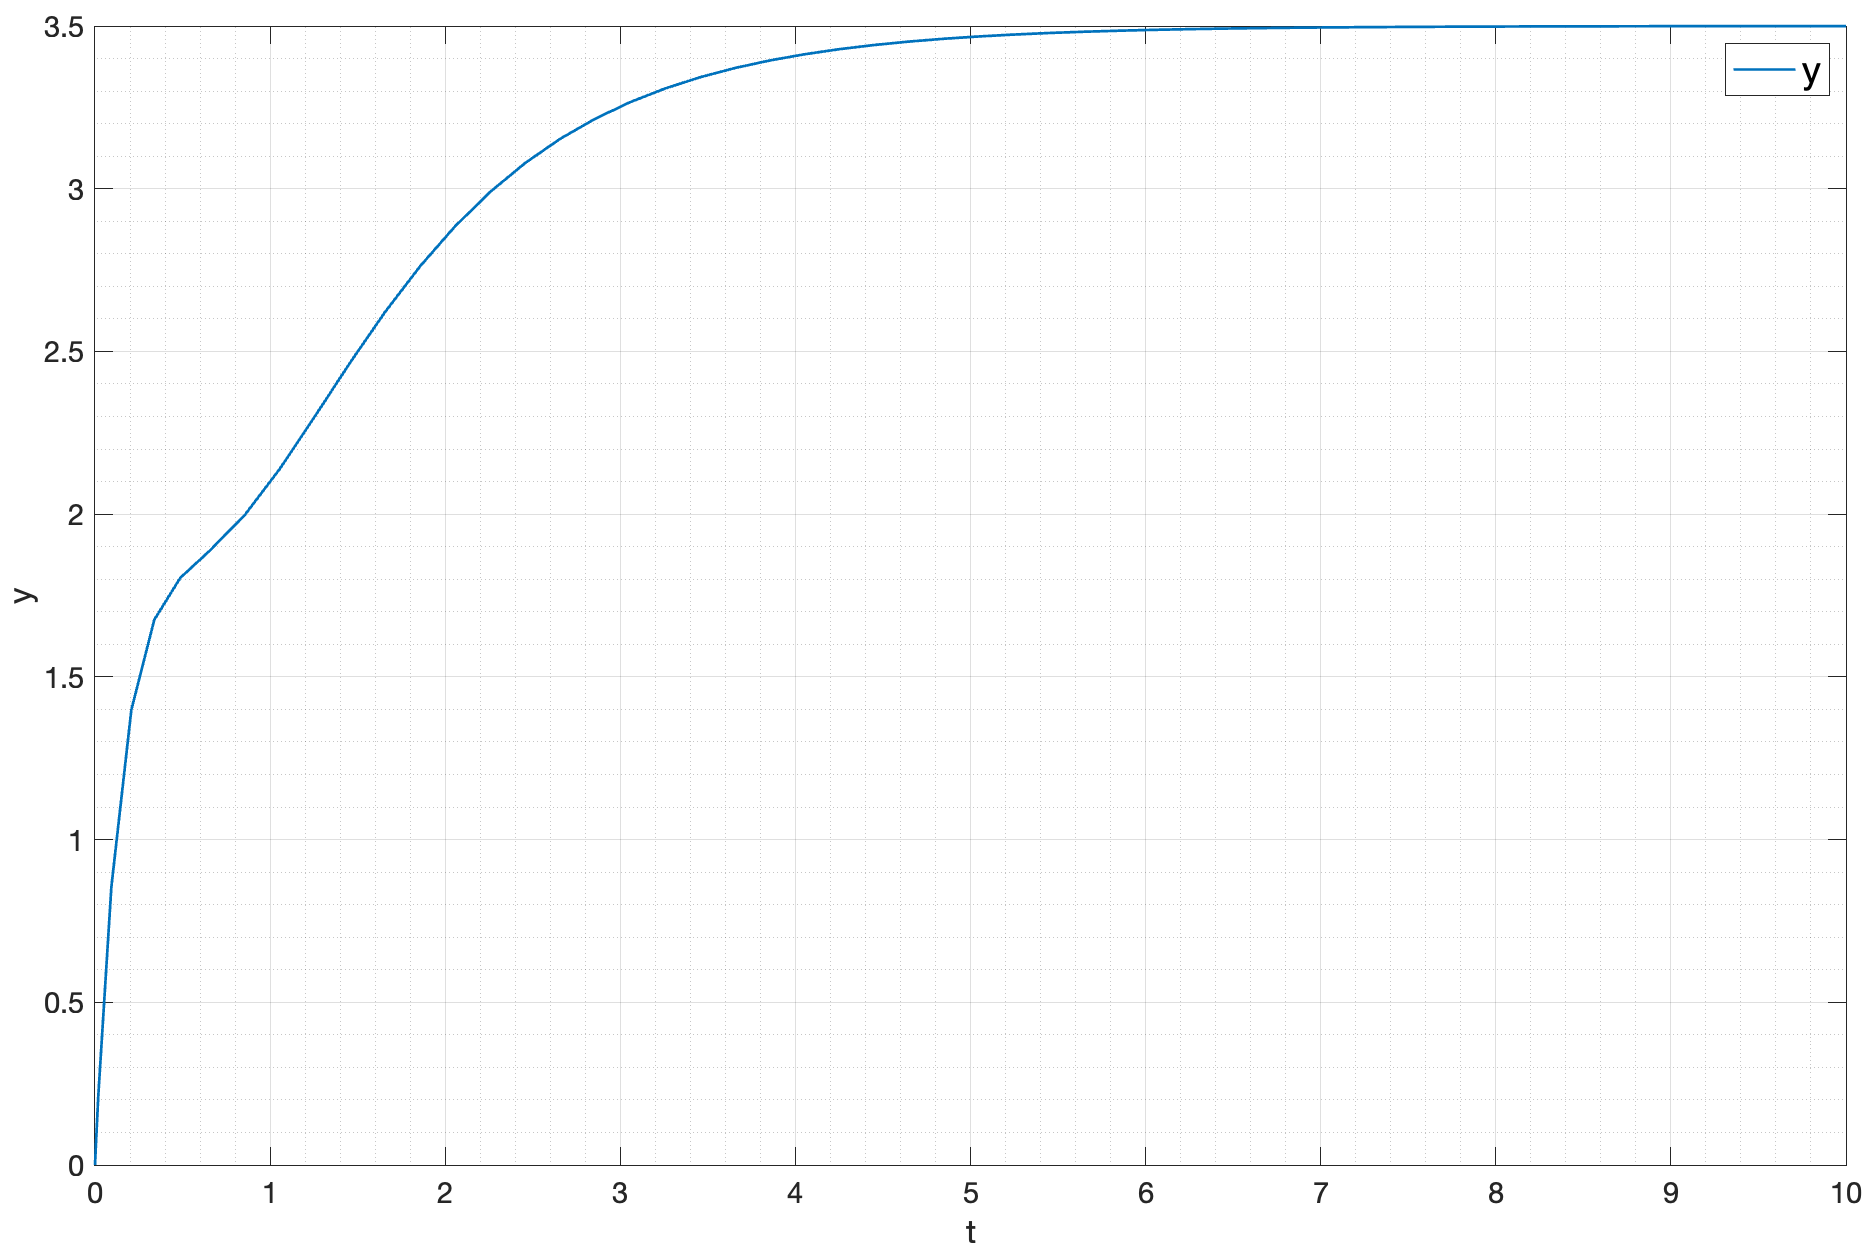
\includegraphics[width=\textwidth]{media/sys3_y(t).png}
    \caption{График $y(t)$}
    \label{fig:yt3}
\end{figure}
\FloatBarrier

На сравнительном графике $y(t)$ для системы в форме В-В и В-С-В (каноническая управляемая форма) (рис. \ref{fig:cmp_sys1_sys3}), видно, что выходные сигналы 
совпадают. 

\begin{figure}[ht!]
    \centering
    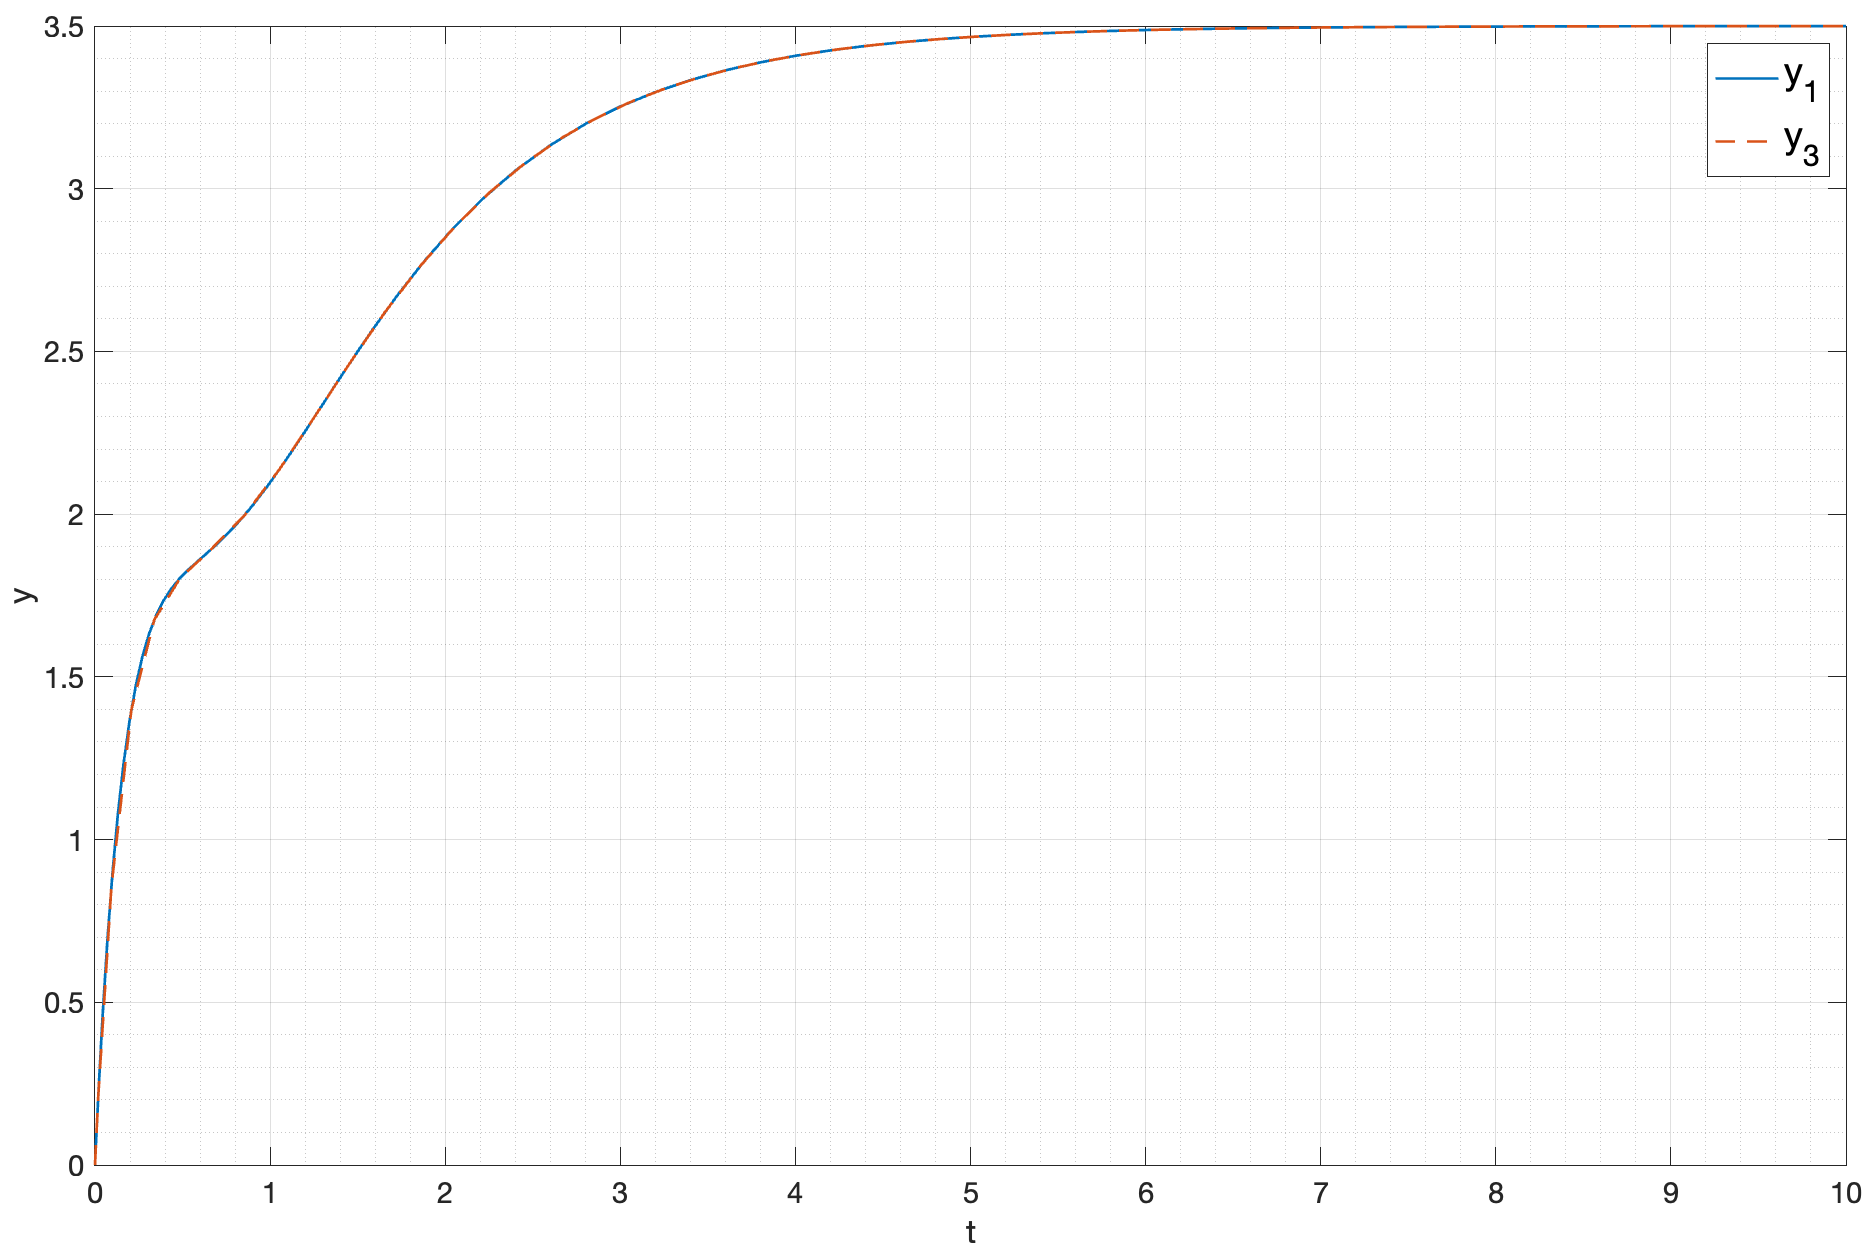
\includegraphics[width=\textwidth]{media/cmp_sys1_sys3.png}
    \caption{Сравнительный график $y(t)$ для системы в форме В-В и В-С-В (каноническая управляемая форма)}
    \label{fig:cmp_sys1_sys3}
    где $y_1(t)$ -- график для системы в форме В-В, $y_2(t)$ -- график для системы в форме В-С-В (каноническая управляемая форма).
\end{figure}


\FloatBarrier
\subsection{Диагональная форма}

Для перехода от формы В-В к форме В-С-В (диагональная форма) воспользуемся следующими соотношениями:
\begin{equation}
    A = \begin{bmatrix}
        \lambda_1 & 0 & 0 \\
        1 & \lambda_2 & 0 \\
        0 & 1 & \lambda_3
    \end{bmatrix},~~~
    B = \begin{bmatrix}
        \beta_1 \\
        \beta_2 \\
        \beta_3
    \end{bmatrix},~~~
    C = \begin{bmatrix}
        \chi_1 & \chi_2 & \chi_3
    \end{bmatrix}
\end{equation}

где $\lambda$, $\beta$, $\chi$ находятся из разложение передаточной функции $W(p)$ на простейшие дроби.
\begin{equation}
    W(p) = \frac{\beta_1\chi_1}{p - \lambda_1} + \frac{\beta_2\chi_2}{p - \lambda_2} + \frac{\beta_3\chi_3}{p - \lambda_3}
\end{equation}

Разложим передаточную функцию $W(p)$ на простейшие дроби:

\begin{equation}
    W(p) = \frac{b_2 p^2 + b_1 p + b_0}{p^3 + a_2 p^2 + a_1 p + a_0} = \frac{12p^2 + 24p + 42}{p^3 + 8p^2 + 19p + 12} = \\
    \frac{A}{p + 1} + \frac{B}{p + 4} + \frac{C}{p + 3}. 
\end{equation}

Найдя коэффициенты $A$, $B$, $C$ методом неопределенных коэффициентов, получим:
\begin{equation}
    W(p) = \frac{5}{p + 1} + \frac{46}{p + 4} + \frac{-39}{p + 3}
\end{equation}

Можно представить в требуемом виде следующим образом: 
\begin{equation}
    W(p) = \frac{1 \cdot 5}{p + 1} + \frac{1 \cdot 46}{p + 4} + \frac{1 \cdot (-39)}{p + 3} 
\end{equation}

Таким образом, получаем следующую систему:
\begin{equation}
    \begin{cases}
        \dot{x}_1 = -x_1 + u\\
        \dot{x}_2 = -4x_2 + u\\
        \dot{x}_3 = -3x_3 - u \\
        y = 5x_1 + 46x_2 - 39x_3
    \end{cases}
\end{equation}


Построим схему моделирования в Matlab Simulink (рис. \ref{fig:model4}).

\begin{figure}[ht!]
    \centering
    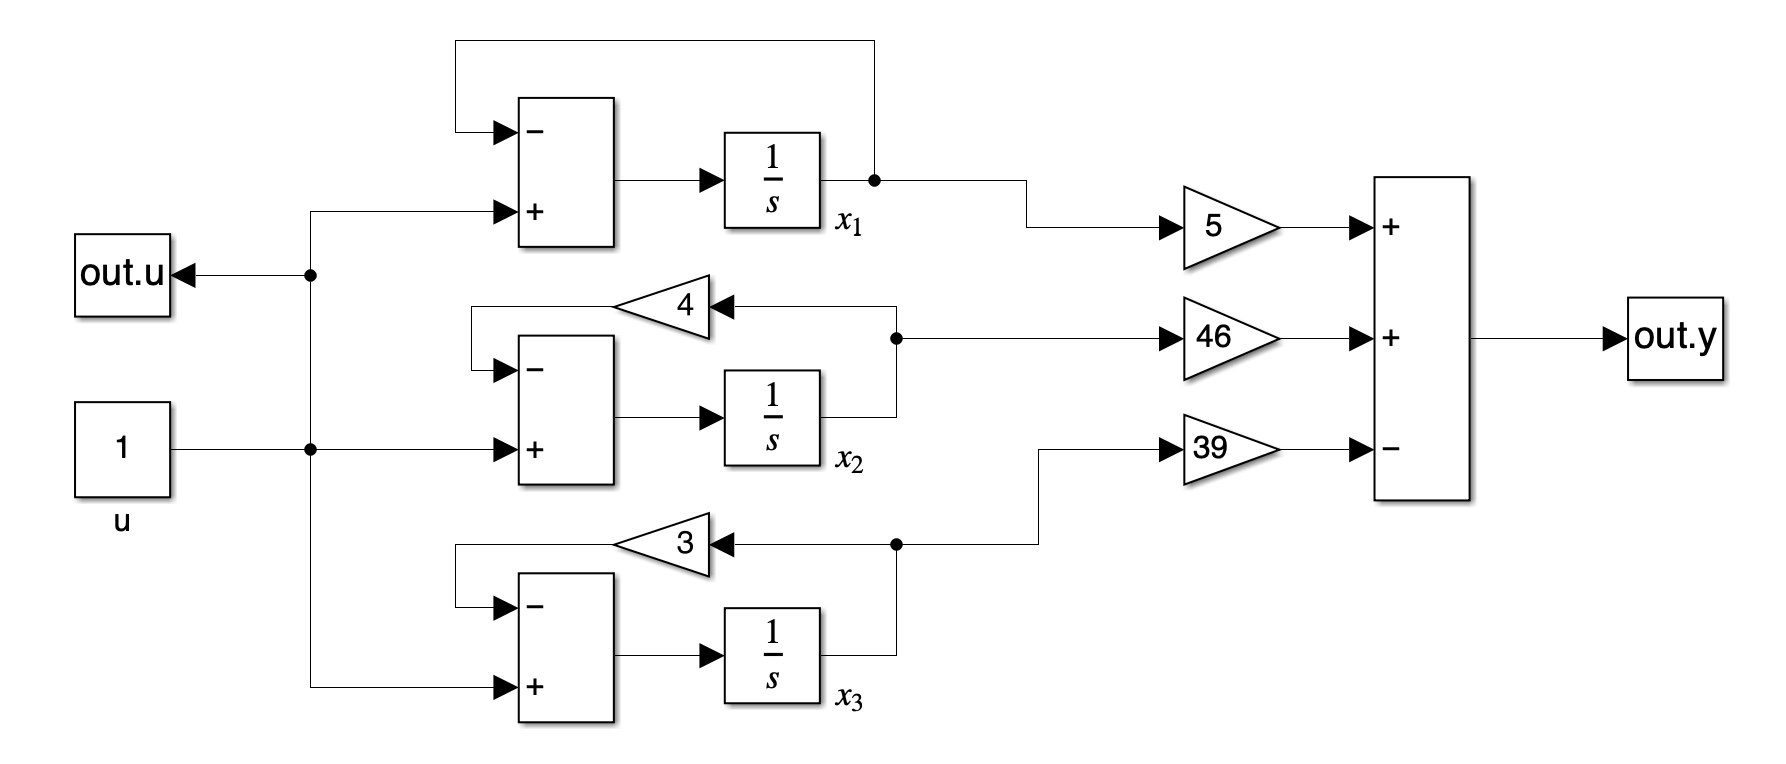
\includegraphics[width=0.7\textwidth]{media/system4.png}
    \caption{Схема моделирования одноканальной системы в форме В-С-В (диагональная форма)}
    \label{fig:model4}
\end{figure}

Промоделировав данную систему получим график $y(t)$ (рис. \ref{fig:yt4}).

\begin{figure}[ht!]
    \centering
    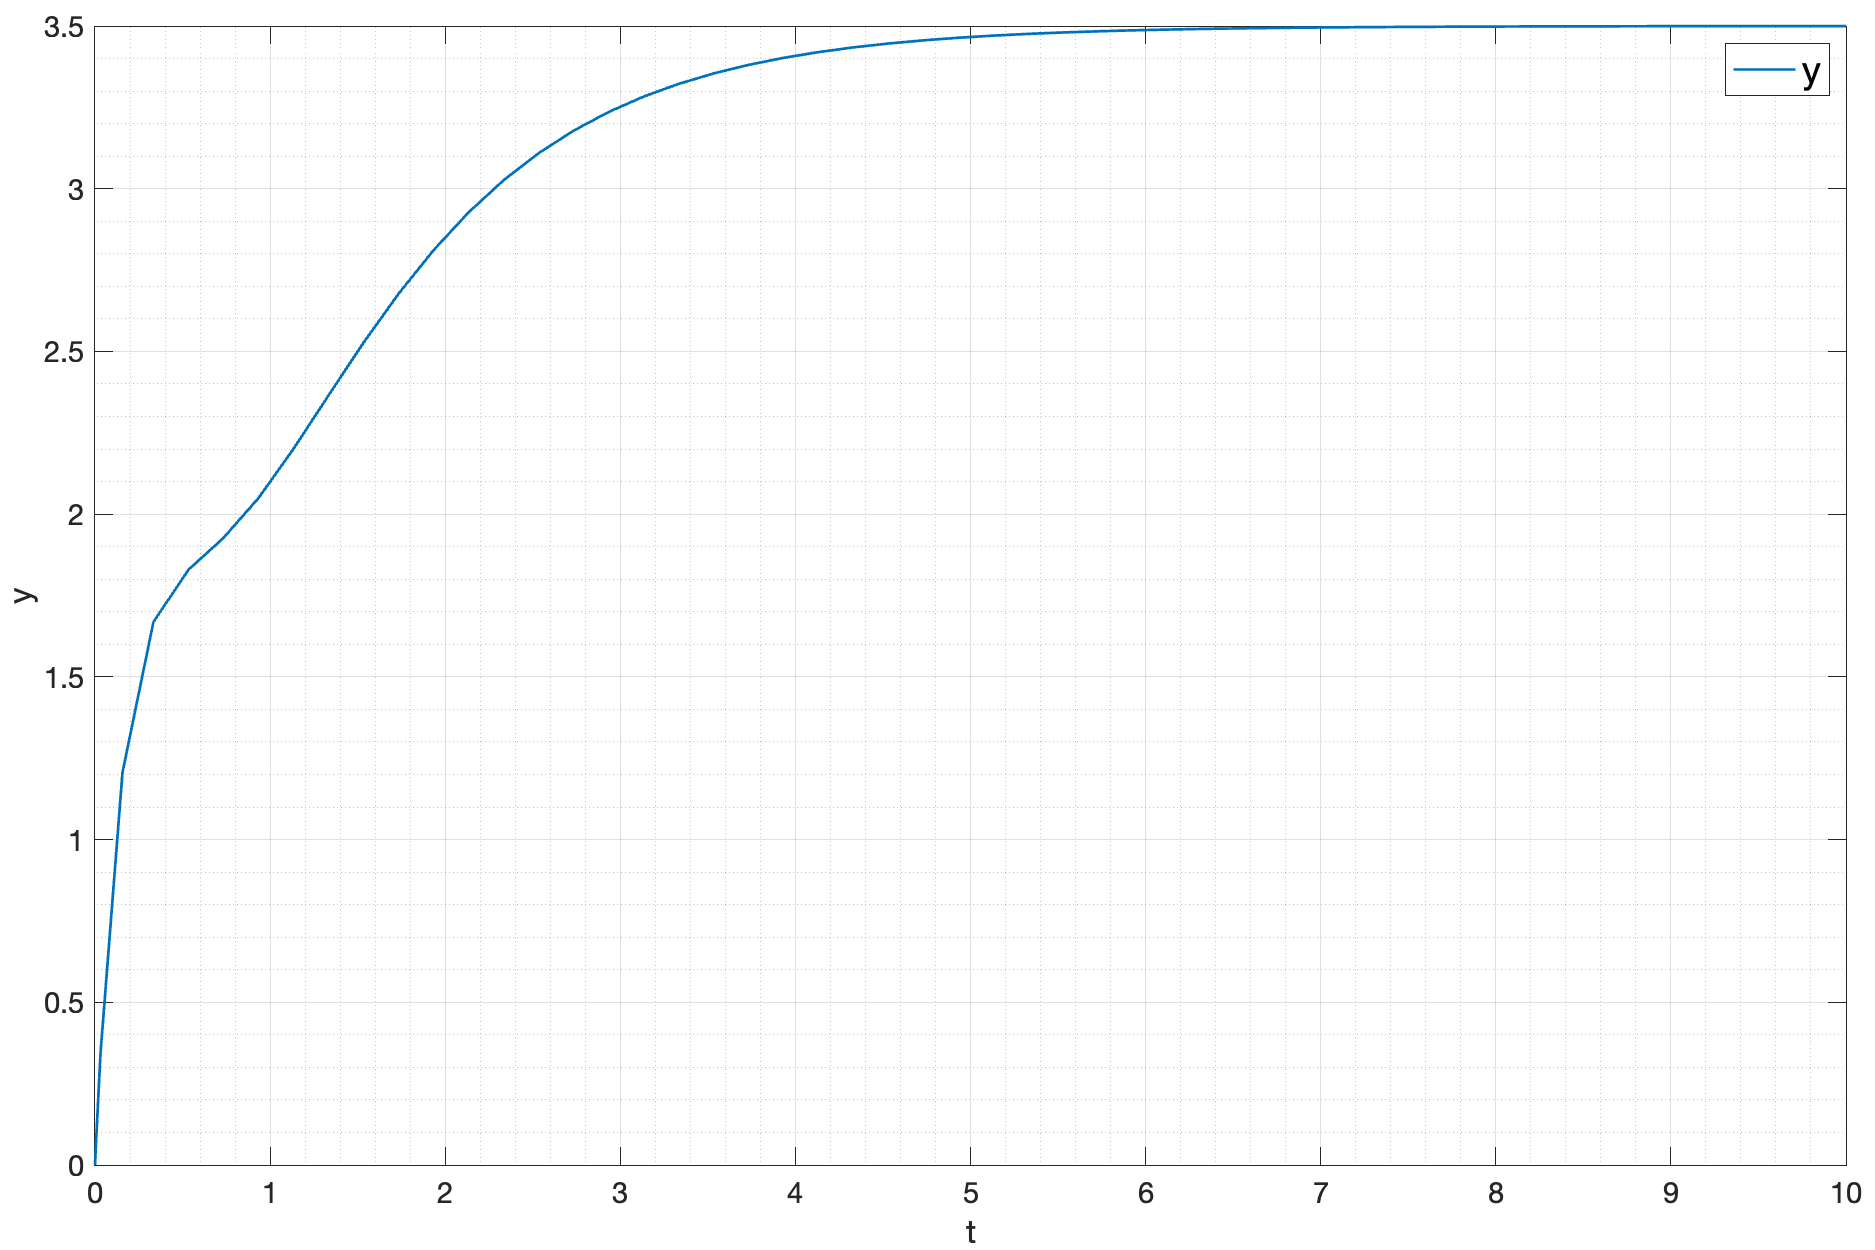
\includegraphics[width=\textwidth]{media/sys4_y(t).png}
    \caption{График $y(t)$}
    \label{fig:yt4}
\end{figure}

На сравнительном графике $y(t)$ для системы в форме В-В и В-С-В (диагональная форма) (рис. \ref{fig:cmp_sys1_sys4}), видно, 
что выходные сигналы совпадают.

\begin{figure}[ht!]
    \centering
    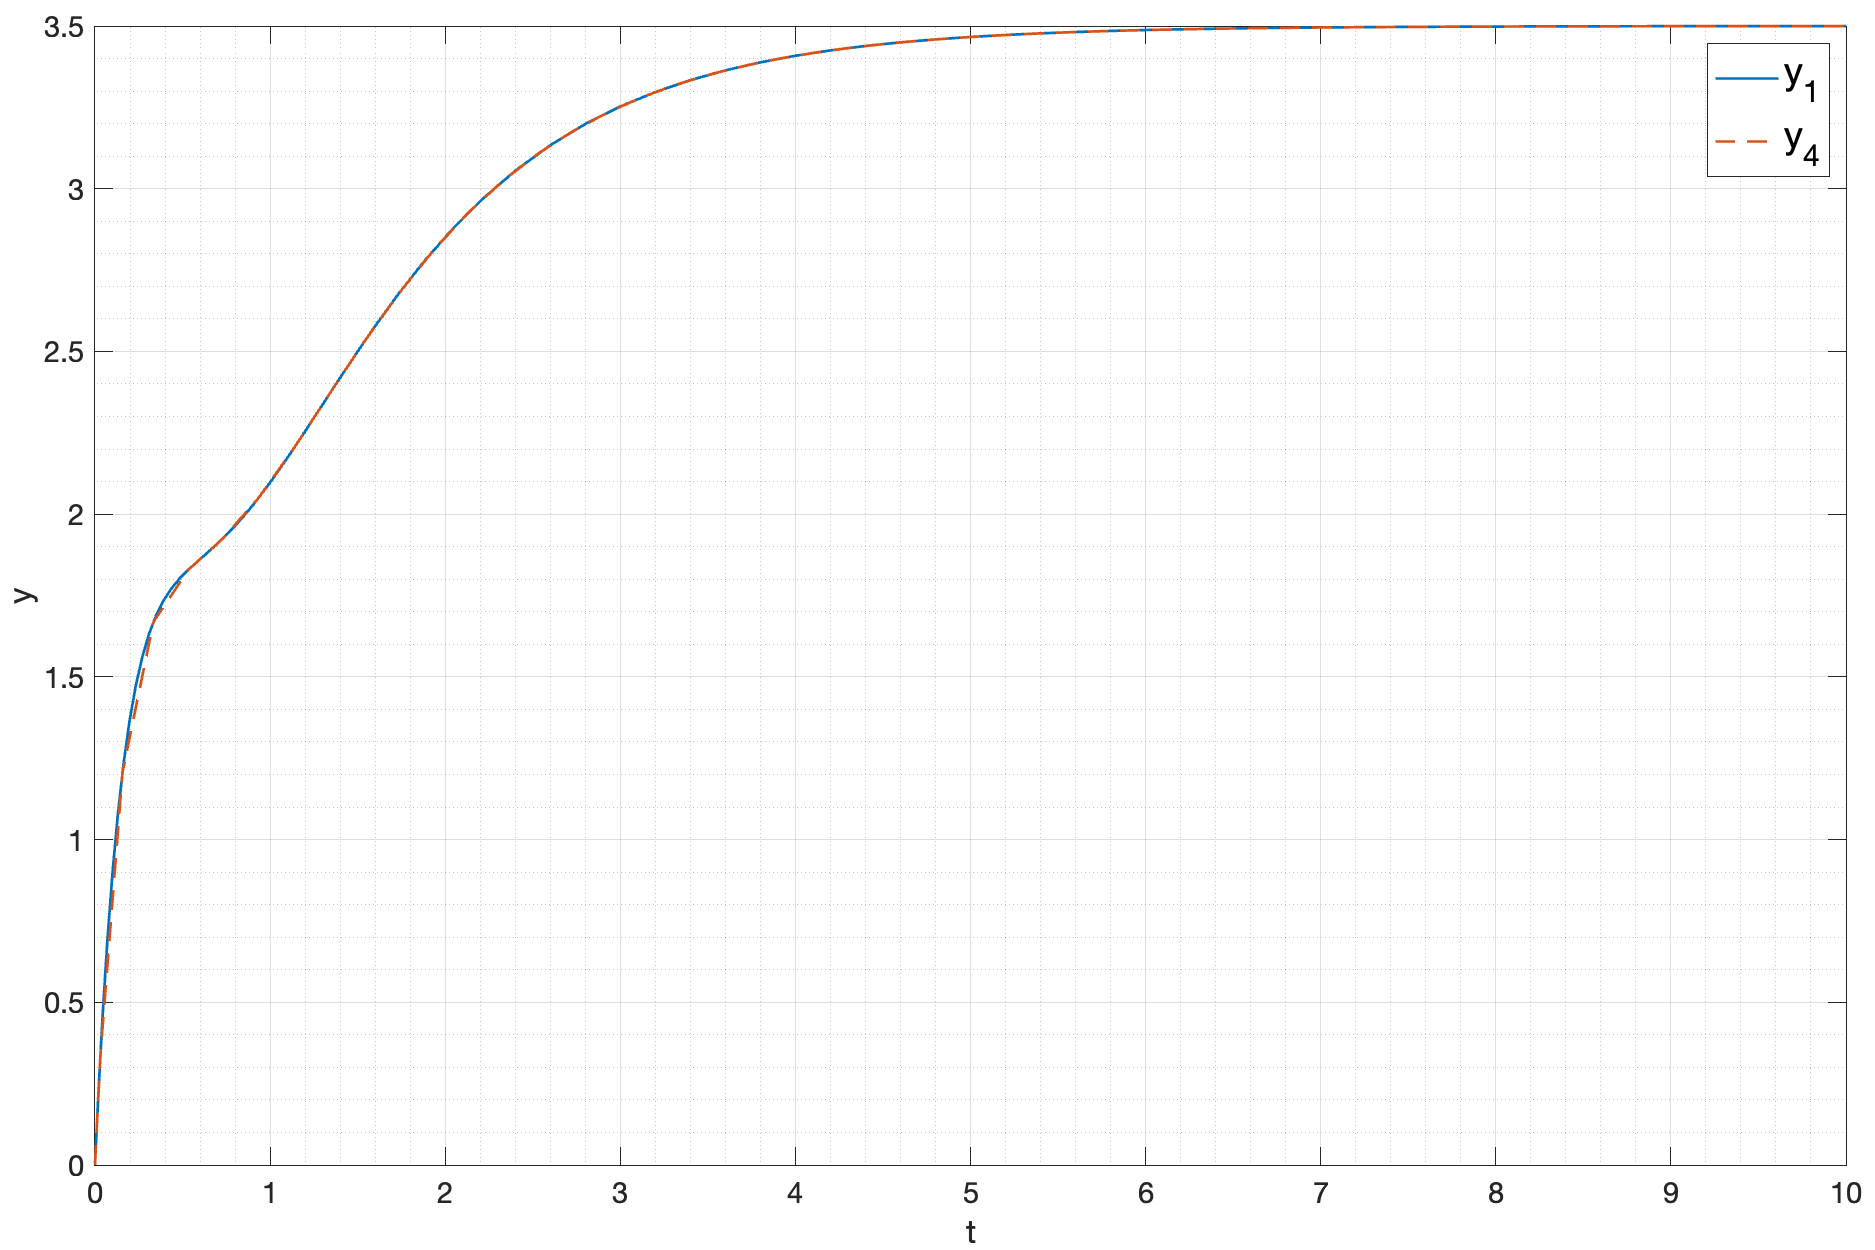
\includegraphics[width=\textwidth]{media/cmp_sys1_sys4.png}
    \caption{Сравнительный график $y(t)$ для системы в форме В-В и В-С-В (диагональная форма)}
    \label{fig:cmp_sys1_sys4}
    где $y_1(t)$ -- график для системы в форме В-В, $y_2(t)$ -- график для системы в форме В-С-В (диагональная форма).
\end{figure}

\FloatBarrier

Таким образом, можно сделать вывод, что одна и та же система может быть представлена в различных формах, но при этом
выходные сигналы будут совпадать (или отличаться только по амплитуде). Кроме того, модель в форме В-С-В позволяет 
оценивать внутреннее состояние системы, что может быть полезно при проектировании систем. 


\FloatBarrier{}

\section{Многоканальная система в форме вход-выход}

Рассмотрим следующую систему: 
\begin{equation}
    A(p) \times y(t) = B(p) \times u(t)
\end{equation}
\begin{equation}
    A = \begin{bmatrix}
        p + 11 & p + 2 \\
        p + 2 & p + 6
    \end{bmatrix},~~~
    B = \begin{bmatrix}
        9 & 8 \\
        1 & 8
    \end{bmatrix}
\end{equation}

Можно выразить $y(t)$ следующим образом:

\begin{equation}
    y(t) = A^{-1}(p) \times B(p) \times u(t)
\end{equation}

При этом сразу появляется выражение для вычисления передаточной матрицы:
\begin{equation}
    W(p) = A^{-1}(p) \times B(p)
\end{equation}

Найдем численные значения: 
\begin{equation}
    A^{-1}(p) = \frac{1}{\det(A)} \times \begin{bmatrix}
        p + 6 & -p - 2 \\
        -p - 2 & p + 11
    \end{bmatrix} = 
    \frac{1}{13p + 62} \times \begin{bmatrix}
        p + 6 & -p - 2 \\
        -p - 1 & p + 11
    \end{bmatrix} = 
    \begin{bmatrix}
        \frac{p + 6}{13p + 62} & \frac{-p - 2}{13p + 62} \\
        \frac{-p - 2}{13p + 62} & \frac{p + 11}{13p + 62}
    \end{bmatrix}
\end{equation}
\begin{equation}
    W(p) = A^{-1}(p) \times B(p) = \begin{bmatrix}
        \frac{8p+52}{13p+62} & \frac{32}{13p+62} \\
        \frac{-8p-7}{13p+62} & \frac{72}{13p+62}
        \end{bmatrix}
\end{equation}

Можно расписать выход в виде:
\begin{equation}
    \begin{bmatrix} 
        y_1(t)\\
        y_2(t)
    \end{bmatrix}
     = \begin{bmatrix}
        \frac{8p+52}{13p+62} & \frac{32}{13p+62} \\
        \frac{-8p-7}{13p+62} & \frac{72}{13p+62}
    \end{bmatrix} \times \begin{bmatrix}
        u_1(t) \\
        u_2(t)
    \end{bmatrix}
\end{equation}

Запишем в виде отдельных уравнений для каждого выхода:
\begin{equation}
    y_1(t) = \frac{8p+52}{13p+62} \times u_1(t) + \frac{32}{13p+62} \times u_2(t)
\end{equation}
\begin{equation}
    y_2(t) = \frac{-8p-7}{13p+62} \times u_1(t) + \frac{72}{13p+62} \times u_2(t)
\end{equation}

Теперь, имея данные уравнения, можно построить схему многоканальной системы в форме вход-выход в среде Simulink.

\begin{figure}
    \centering
    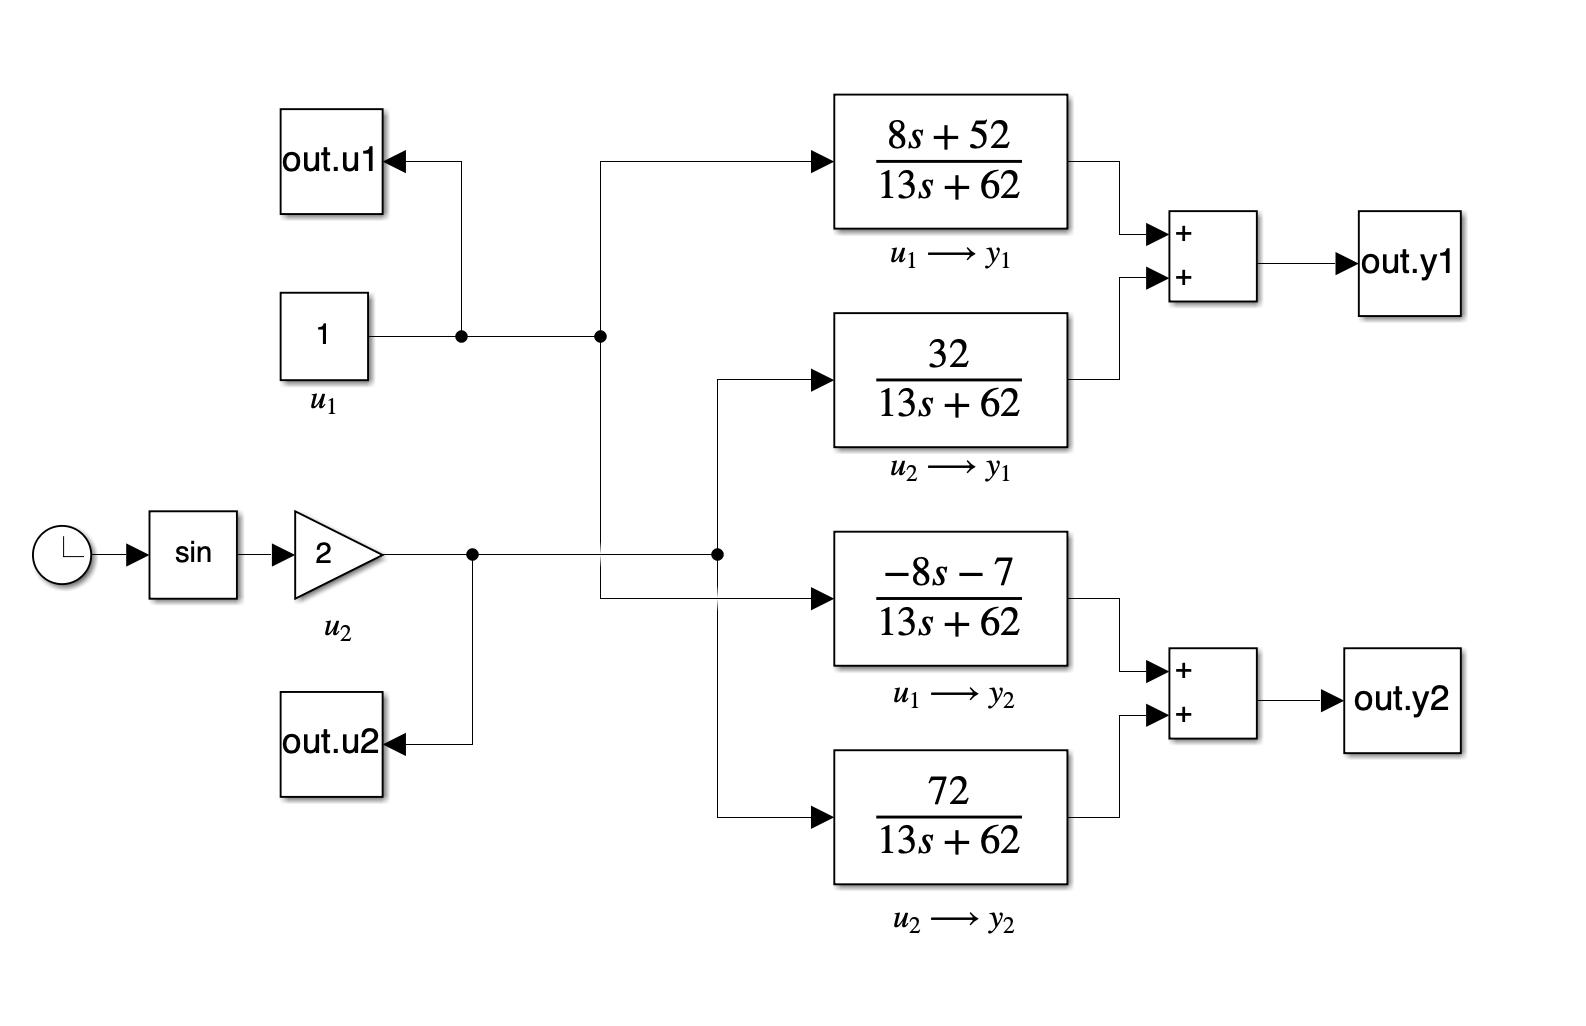
\includegraphics[width=0.8\textwidth]{media/system5.png}
    \caption{Схема многоканальной системы в форме вход-выход}
    \label{fig:MultyChannel}
\end{figure}

Промоделировав данную систему, получим графики $y_1(t)$ и $y_2(t)$, $u_1(t)$ и $u_2(t)$.

\begin{figure}[ht!]
    \centering
    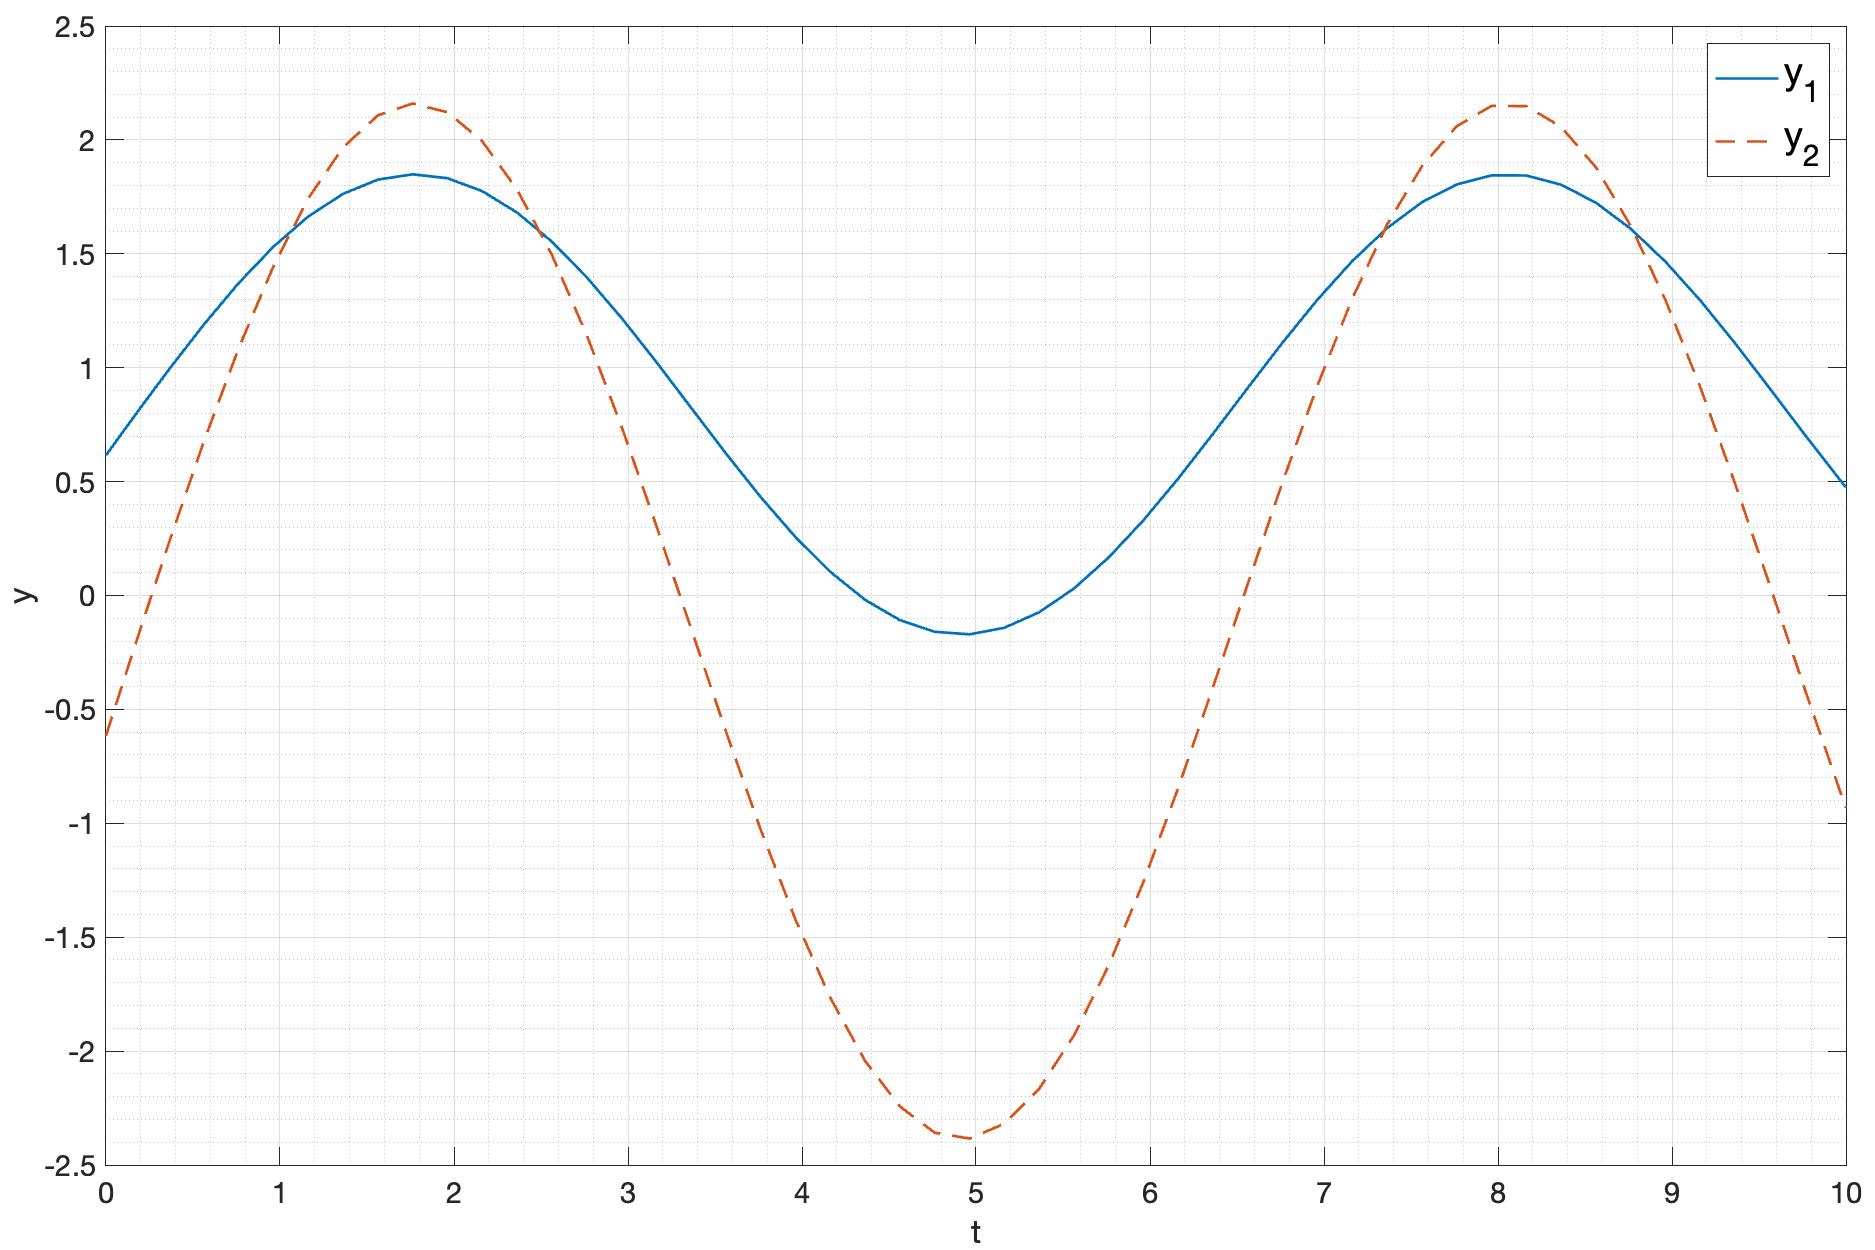
\includegraphics[width=\textwidth]{media/sys5_y(t).png}
    \caption{Графики $y_1(t)$ и $y_2(t)$}
    \label{fig:yt5}
\end{figure}

\begin{figure}[ht!]
    \centering
    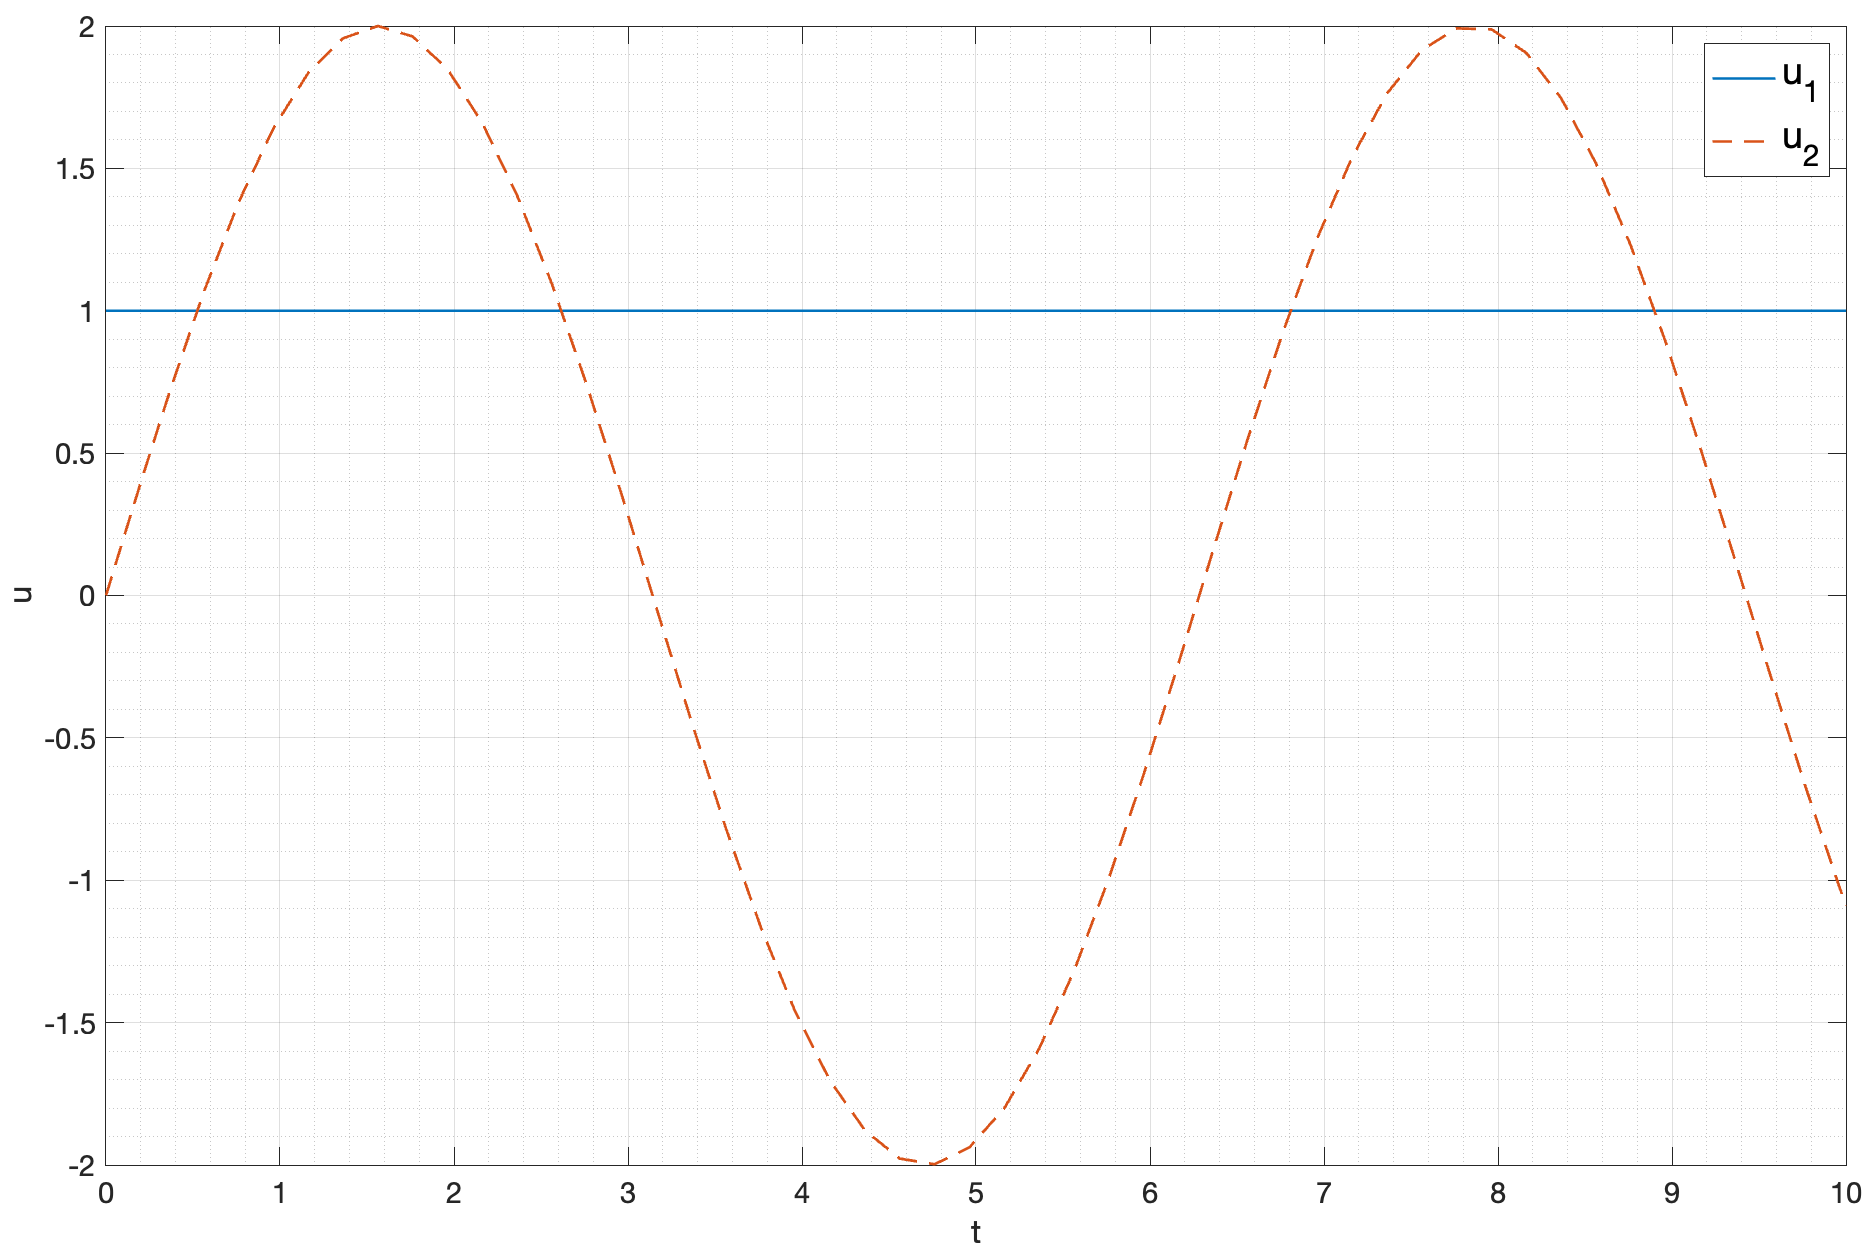
\includegraphics[width=\textwidth]{media/sys5_u(t).png}
    \caption{Графики $u_1(t)$ и $u_2(t)$}
    \label{fig:ut5}
\end{figure}

\FloatBarrier
\section{Многоканальная система в форме вход-состояние-выход}

Рассмотрим следующую систему:
\begin{equation}
    \begin{cases}
        \dot{x}(t) = A x + B u \\
        y(t) = Cx
    \end{cases}
\end{equation}

\begin{equation}
    A = \begin{bmatrix}
        0 & -9 \\
        1 & -3
    \end{bmatrix},~~~
    B = \begin{bmatrix}
        9 & 5 \\
        2 & 11
    \end{bmatrix},~~~
    C = \begin{bmatrix}
        5 & 6 \\
        3 & 8
    \end{bmatrix}
\end{equation}

Распишем систему в виде уравнений:
\begin{equation}
    \begin{cases}
        \dot{x}_1 = -9x_2 + -9u_1 + 5u_2 \\
        \dot{x}_2 = x_1 - 3x_2 + 2u_1 + 11u_2 \\
        y_1 = 5x_1 + 6x_2 \\
        y_2 = 3x_1 + 8x_2
    \end{cases}
\end{equation}

Теперь построим схему моделирования в Simulink.

\begin{figure}[ht!]
    \centering
    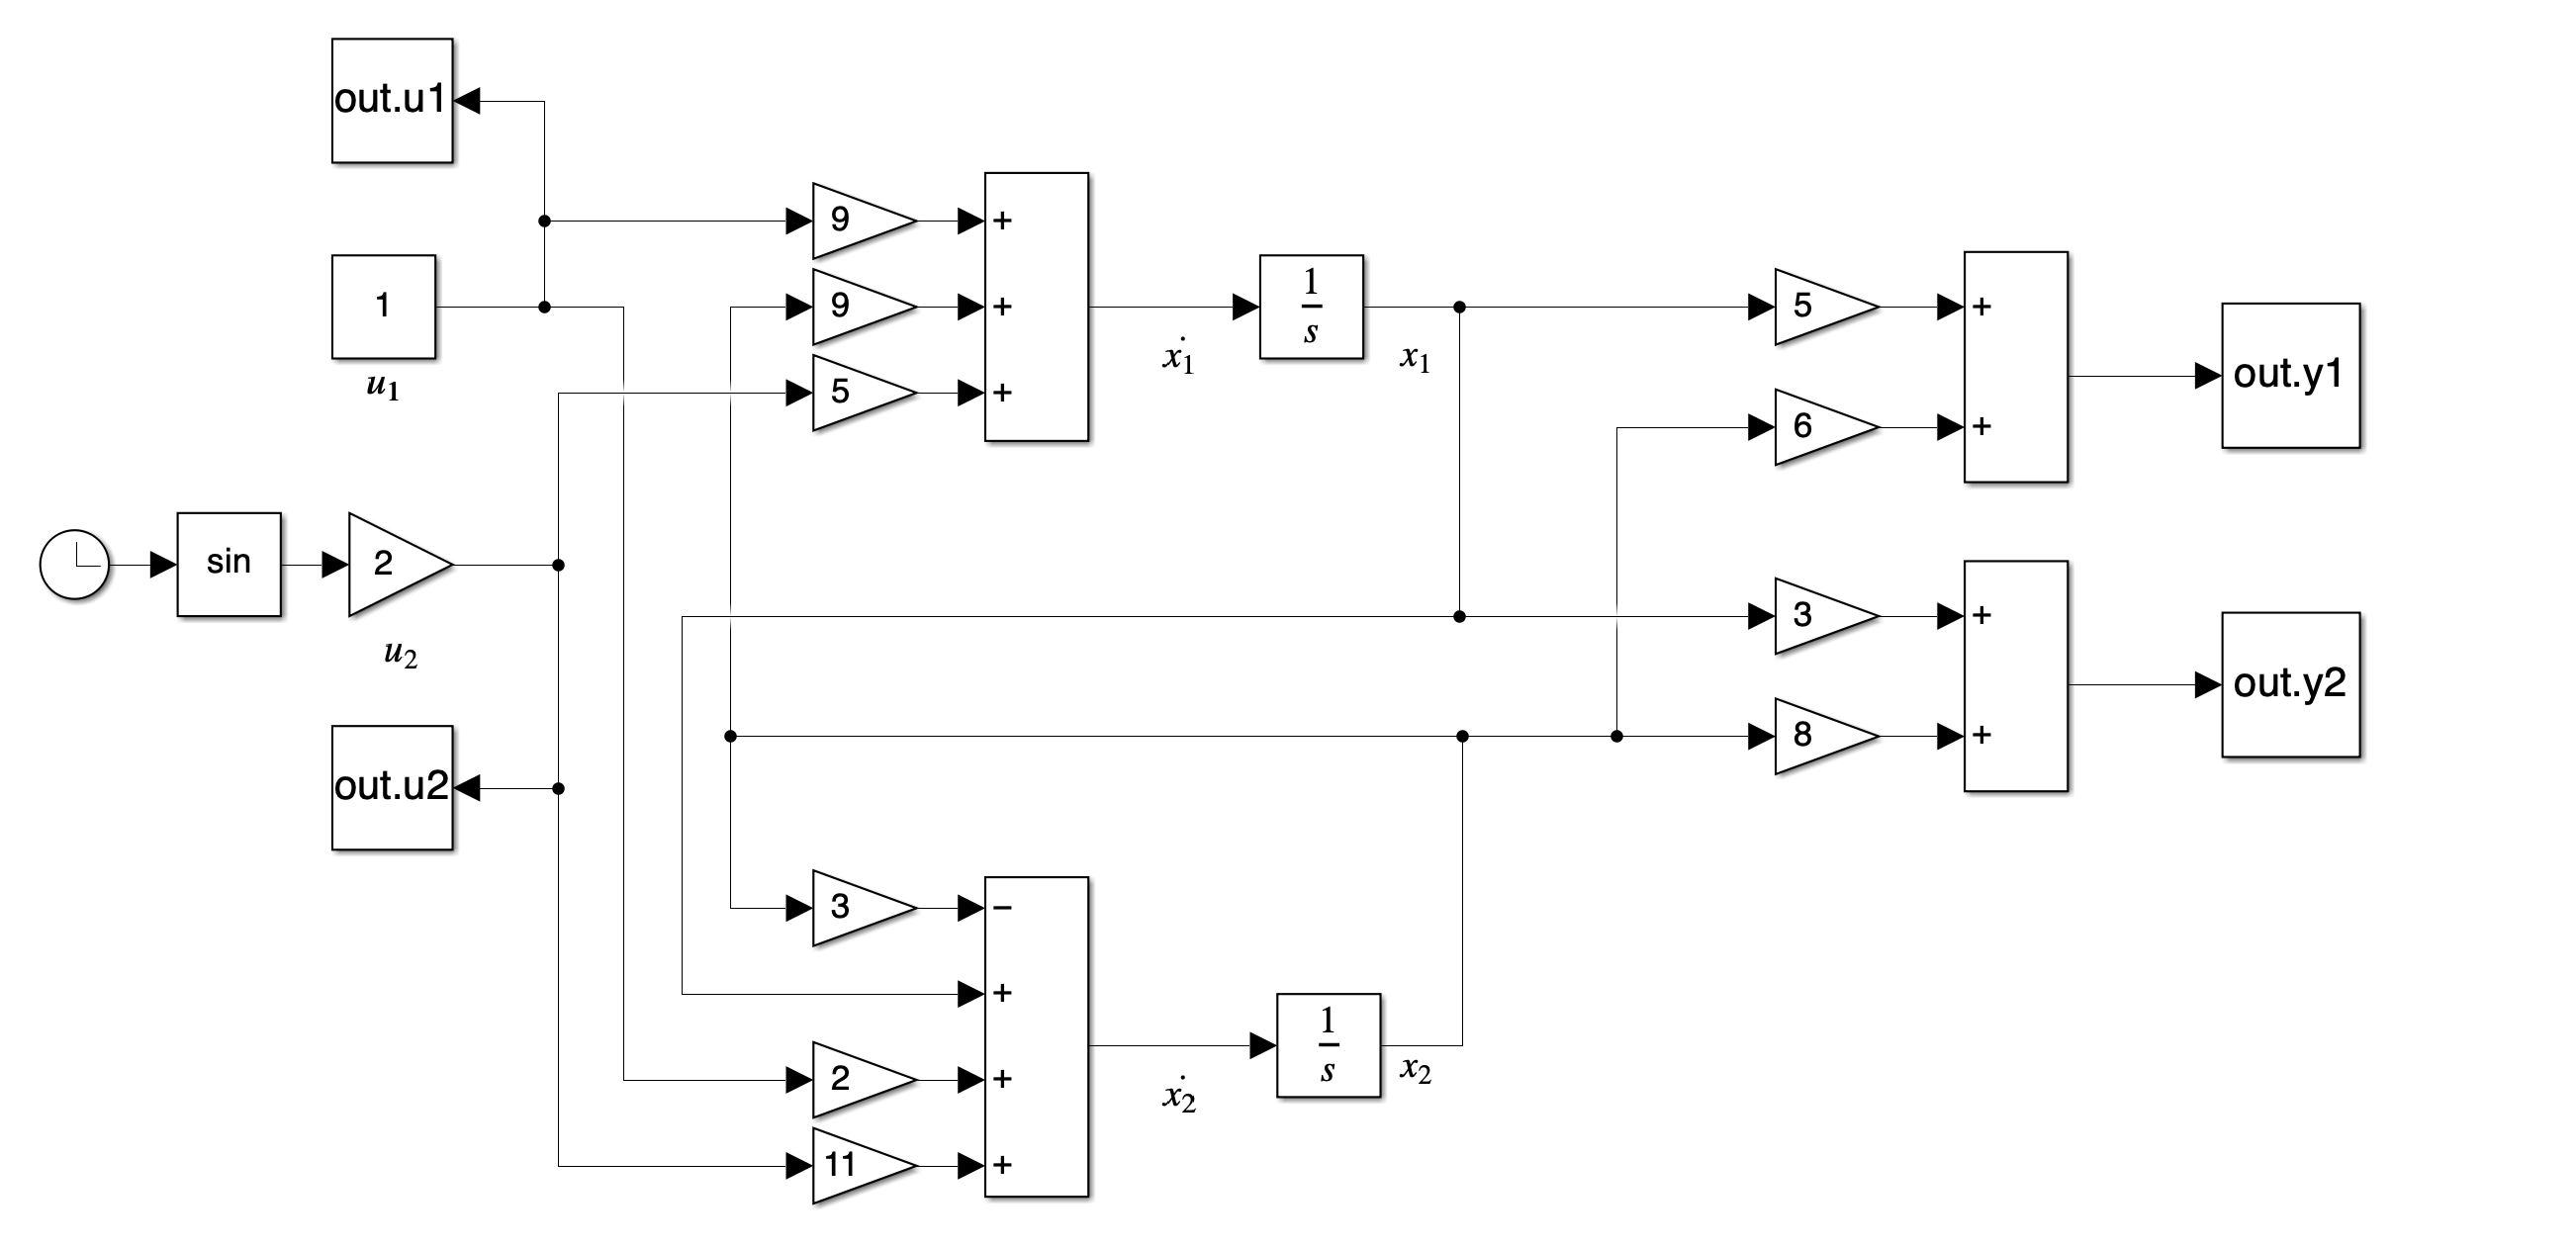
\includegraphics[width=0.8\textwidth]{media/system6.png}
    \caption{Схема многоканальной системы в форме вход-состояние-выход}
    \label{fig:model6}
\end{figure}

Промоделировав данную систему, получим графики $y_1(t)$ и $y_2(t)$, $u_1(t)$ и $u_2(t)$.

\begin{figure}[ht!]
    \centering
    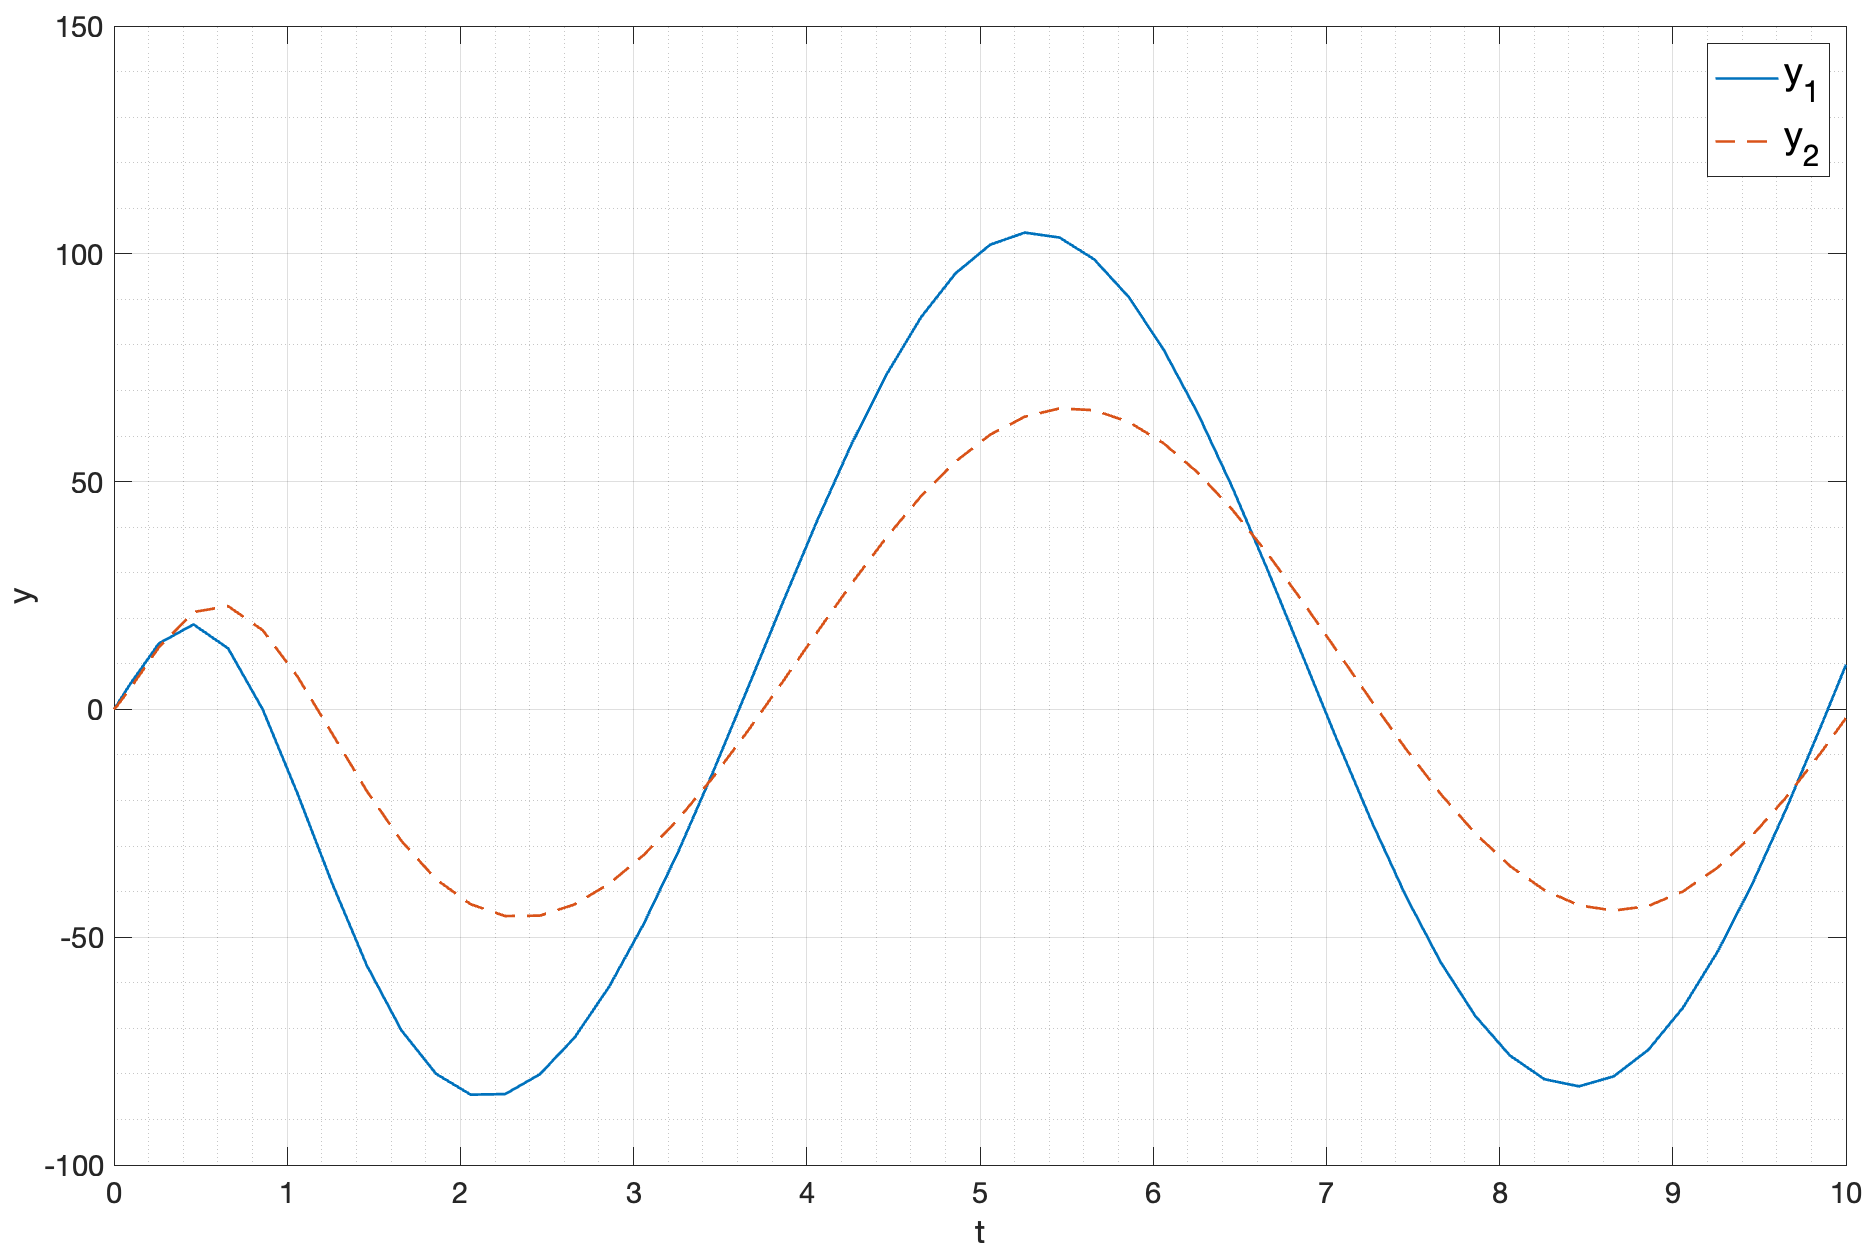
\includegraphics[width=\textwidth]{media/sys6_y(t).png}
    \caption{Графики $y_1(t)$ и $y_2(t)$}
    \label{fig:yt6}
\end{figure}

\begin{figure}[ht!]
    \centering
    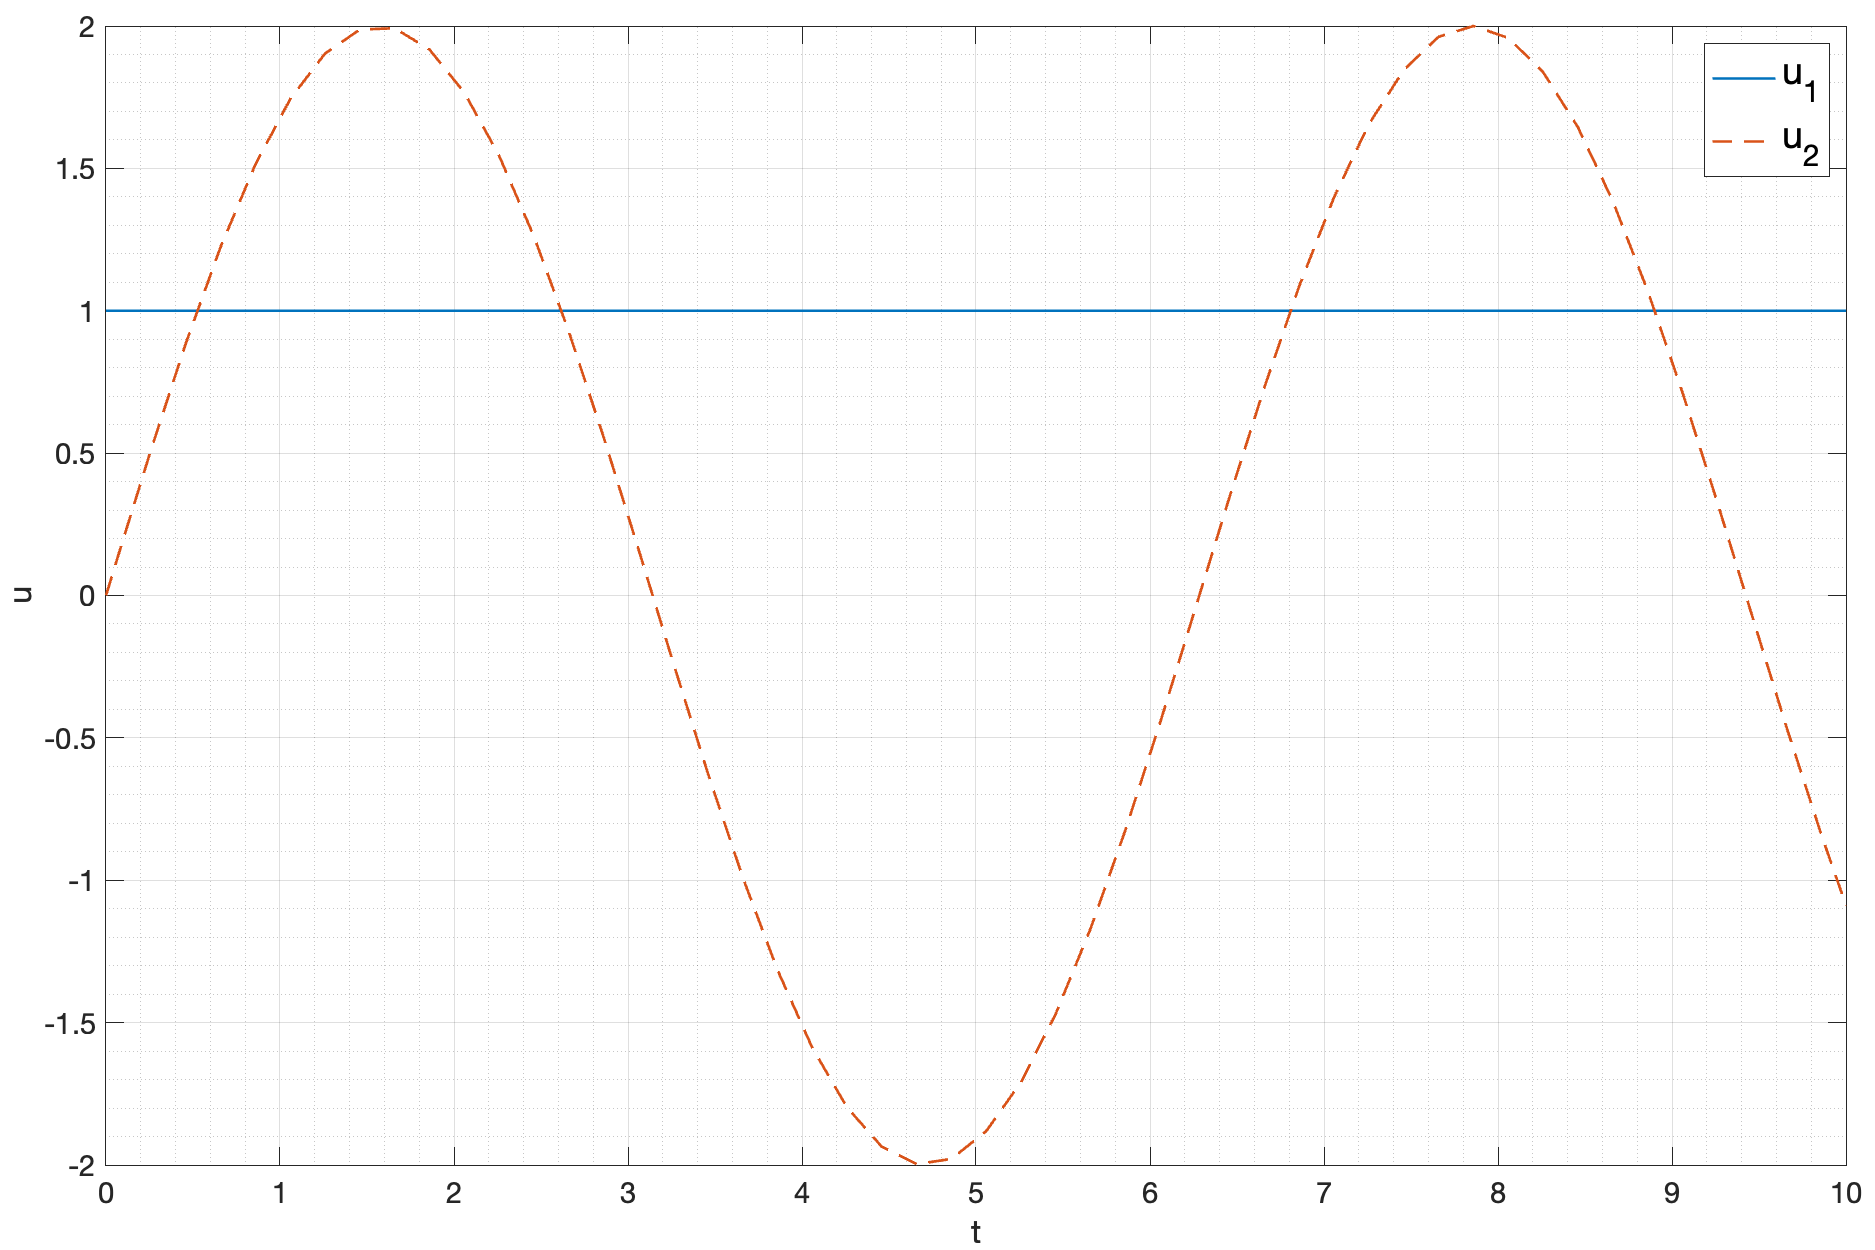
\includegraphics[width=\textwidth]{media/sys6_u(t).png}
    \caption{Графики $u_1(t)$ и $u_2(t)$}
    \label{fig:ut6}
\end{figure}
\FloatBarrier{}

\section{Выводы}
В первом и втором задании рассматривались системы в форме вход-выход и вход-состояние-выход 
(каноническая наблюдаемая форма, каноническая управляемая форма и диагональная форма). 
В каждом из этих вариантов были получены идентичные (за исключением амплитуды) выходные сигналы,
что подтверждает то, что одна и та же система может быть представлена множеством различных форм. 

Кроме того, были рассмотрены многоканальные системы, которые удалось разбить на несколько 
одноканальных систем, что позволило упростить моделирование системы. 